%%%%%%%%%%%%%%%%%%%%%%%%%%%%%%%%%%%%%%%%%
% Masters Thesis 
% LaTeX Template
%
% This template is based on a template by:
% Steve Gunn (http://users.ecs.soton.ac.uk/srg/softwaretools/document/templates/)
% Sunil Patel (http://www.sunilpatel.co.uk/thesis-template/)
%
% Template license:
% CC BY-NC-SA 3.0 (http://creativecommons.org/licenses/by-nc-sa/3.0/)
%
%%%%%%%%%%%%%%%%%%%%%%%%%%%%%%%%%%%%%%%%%

%----------------------------------------------------------------------------------------
%	PACKAGES AND OTHER DOCUMENT CONFIGURATIONS
%----------------------------------------------------------------------------------------

\documentclass[
11pt, % The default document font size, options: 10pt, 11pt, 12pt
%oneside, % Two side (alternating margins) for binding by default, uncomment to switch to one side
english, % ngerman for German
onehalfspacing, % Single line spacing, alternatives: onehalfspacing or doublespacing
%draft, % Uncomment to enable draft mode (no pictures, no links, overfull hboxes indicated)
%nolistspacing, % If the document is onehalfspacing or doublespacing, uncomment this to set spacing in lists to single
%liststotoc, % Uncomment to add the list of figures/tables/etc to the table of contents
%toctotoc, % Uncomment to add the main table of contents to the table of contents
%parskip, % Uncomment to add space between paragraphs
%nohyperref, % Uncomment to not load the hyperref package
headsepline, % Uncomment to get a line under the header
%chapterinoneline, % Uncomment to place the chapter title next to the number on one line
%consistentlayout, % Uncomment to change the layout of the declaration, abstract and acknowledgements pages to match the default layout
]{MastersDoctoralThesis} % The class file specifying the document structure

\usepackage[utf8]{inputenc} % Required for inputting international characters
\usepackage[T1]{fontenc} % Output font encoding for international characters

\usepackage{mathpazo} % Use the Palatino font by default

\usepackage[backend=bibtex,style=authoryear,natbib=true]{biblatex} % Use the bibtex backend with the authoryear citation style (which resembles APA)

\addbibresource{references.bib} % The filename of the bibliography

% --- Citation style: square-bracket author-year with "et al." (match reference TFM) ---
\ExecuteBibliographyOptions{maxcitenames=2,mincitenames=1}
\renewcommand*{\nameyeardelim}{\addcomma\space} % renders as [Author, year]
\DeclareCiteCommand{\parencite}[\mkbibbrackets]
  {\usebibmacro{prenote}}
  {\usebibmacro{citeindex}\usebibmacro{cite}}
  {\multicitedelim}
  {\usebibmacro{postnote}}
\let\autocite\parencite
\let\textcite\parencite % bracket subject-citations too, as in the reference thesis

% --- Hyperlink colours (match reference TFM) ---
\definecolor{linkcol}{HTML}{1B7F79} % teal: internal cross-references
\definecolor{citecol}{HTML}{B5179E} % magenta: citations
\definecolor{urlcol}{HTML}{7B241C}  % maroon: URLs / DOIs

\usepackage[autostyle=true]{csquotes} % Required to generate language-dependent quotes in the bibliography

\usepackage{amsmath} % Mathematical symbols and environments
\usepackage{amssymb} % Additional math symbols (\mathbb, etc.)
\usepackage{booktabs} % Better table formatting
\usepackage{graphicx} % Enhanced graphics support
\usepackage{caption} % Better caption control
\usepackage{subcaption} % Sub-figures
\usepackage{tikz} % Pipeline diagram in Chapter 3

\emergencystretch=2em % Allow whitespace stretch to avoid overfull hboxes
\tolerance=1500 % Slightly more tolerant line breaking

%----------------------------------------------------------------------------------------
%	MARGIN SETTINGS
%----------------------------------------------------------------------------------------

\geometry{
	paper=a4paper, % Change to letterpaper for US letter
	inner=2.5cm, % Inner margin
	outer=3.8cm, % Outer margin
	bindingoffset=.5cm, % Binding offset
	top=1.5cm, % Top margin
	bottom=1.5cm, % Bottom margin
	%showframe, % Uncomment to show how the type block is set on the page
}

%----------------------------------------------------------------------------------------
%	THESIS INFORMATION
%----------------------------------------------------------------------------------------

\thesistitle{Data-Driven Cognitive Phenotyping in Acquired Brain Injury: A Clustering Analysis with Imputation Robustness Assessment} % Your thesis title
\supervisor{Dr.\ Alejandro García-Rudolph} % Your supervisor's name
\examiner{} % Your examiner's name
\degree{MSc} % Your degree name
\author{Zoltan Kunos} % Your name
\addresses{} % Your address

\subject{Data Science} % Your subject area
\keywords{acquired brain injury, cognitive phenotyping, clustering, UMAP, HDBSCAN, missing data imputation, neuropsychology} % Keywords
\university{\href{http://www.ub.edu}{Universitat de Barcelona}} % Your university's name and URL, this is used in the title page and abstract, print it elsewhere with \univname
\department{\href{http://department.university.com}{}} % Your department's name and URL, this is used in the title page and abstract, print it elsewhere with \deptname
\group{\href{http://researchgroup.university.com}{}} % Your research group's name and URL, this is used in the title page, print it elsewhere with \groupname
\faculty{\href{http://mat.ub.edu}{Facultat de Matemàtiques i Informàtica}} % Your faculty's name and URL, this is used in the title page and abstract, print it elsewhere with \facname

\AtBeginDocument{
\hypersetup{pdftitle=\ttitle} % Set the PDF's title to your title
\hypersetup{pdfauthor=\authorname} % Set the PDF's author to your name
\hypersetup{pdfkeywords=\keywordnames} % Set the PDF's keywords to your keywords
\hypersetup{linkcolor=linkcol} % Teal cross-references
\hypersetup{citecolor=citecol} % Magenta citations
\hypersetup{urlcolor=urlcol} % Maroon URLs / DOIs
}

\begin{document}

\frontmatter % Use roman page numbering style (i, ii, iii, iv...) for the pre-content pages

\pagestyle{plain} % Default to the plain heading style until the thesis style is called for the body content

%----------------------------------------------------------------------------------------
%	TITLE PAGE
%----------------------------------------------------------------------------------------

\begin{titlepage}
\begin{center}

\vspace*{.06\textheight}
{\scshape\LARGE \univname\par}\vspace{1.5cm} % University name
\textsc{\Large Fundamental Principles of Data Science Master's Thesis}\\[0.5cm] % Thesis type

\HRule \\[0.4cm] % Horizontal line
{\huge \bfseries \ttitle\par}\vspace{0.4cm} % Thesis title
\HRule \\[1.5cm] % Horizontal line
 
\begin{minipage}[t]{0.4\textwidth}
\begin{flushleft} \large
\emph{Author:}\\
\href{http://www.johnsmith.com}{\authorname} % Author name - remove the \href bracket to remove the link
\end{flushleft}
\end{minipage}
\begin{minipage}[t]{0.4\textwidth}
\begin{flushright} \large
\emph{Supervisor:} \\
\href{http://www.jamessmith.com}{\supname} % Supervisor name - remove the \href bracket to remove the link  
\end{flushright}
\end{minipage}\\[3cm]
 
\vfill

\large \textit{A thesis submitted in partial fulfillment of the requirements\\ for the degree of MSc in Fundamental Principles of Data Science}\\[0.3cm] % University requirement text
\textit{in the}\\[0.4cm]
\facname\\[2cm] % Research group name and department name
 
\vfill

{\large \today}\\[4cm] % Date
%\includegraphics{Logo} % University/department logo - uncomment to place it
 
\vfill
\end{center}
\end{titlepage}


%----------------------------------------------------------------------------------------
%	ABSTRACT PAGE
%----------------------------------------------------------------------------------------

\begin{abstract}[]
\addchaptertocentry{\abstractname}
Following acquired brain injury (ABI), cognitive performance is among the strongest predictors of long-term functional outcome. The patients most likely to require intensive rehabilitation, however, are often the least likely to complete a full neuropsychological battery. Missingness in this setting is therefore clinically informative: fatigue, confusion, motor limitation, test tolerance, and examiner judgement all constrain which measures are administered. A complete-case analysis would preferentially retain healthier assessments and discard many of the most impaired patients. Broad diagnostic categories and injury-severity bands introduce a second limitation, since neither captures the cognitive variation needed for personalised rehabilitation planning.

This thesis addresses these problems by pairing missing-data imputation with unsupervised clustering. Incomplete assessments are retained, cognitive structure is inferred directly from test data, and the dependence of that structure on the selected imputation method is evaluated explicitly.

The analysis used 17,406 neuropsychological assessments from 7,285 patients with ABI. It recovered a three-tier cognitive structure: \emph{Above-Average} (38.6\%, $n = 6{,}725$), \emph{Near-Normal} (36.4\%, $n = 6{,}328$), and \emph{Global Impairment} (25\%, $n = 4{,}353$). The tiers differ primarily in overall cognitive level rather than profile shape. All six cognitive domains co-vary across the tiers, and one severity factor explains 56\% of their shared variance. The clusters are therefore better interpreted as a data-driven cognitive-severity continuum than as qualitatively distinct phenotypes. No attention-specific dissociation was supported.

The severity structure was stable across imputation strategies. Under the pre-registered criteria, all ten methods yielded distinct, low-noise solutions, with a mean pairwise Adjusted Rand Index (ARI) of 0.71. The primary MICE solution achieved a full-coverage silhouette of 0.526 and no residual noise points. Tier membership was also associated with clinical-unit placement after adjustment for diagnosis (Cram\'{e}r's V 0.16; Cochran-Mantel-Haenszel test), indicating that the recovered structure corresponds to clinically meaningful patient routing rather than to a purely methodological artefact. Domain-level aggregation further improved numerical conditioning relative to variable-level clustering, reducing the mean VIF from 2.8 to 1.9 and the condition number from 62 to 12.

CogDash, the accompanying interactive dashboard, implements the full pipeline for future patients and reports both severity tier and consensus confidence across imputation methods. The code, notebooks, and dashboard are available at \url{https://github.com/zkunos/thesis_project}.
\end{abstract}

%----------------------------------------------------------------------------------------
%	ACKNOWLEDGEMENTS
%----------------------------------------------------------------------------------------

\begin{acknowledgements}
\addchaptertocentry{\acknowledgementname} % Add the acknowledgements to the table of contents
My deepest thanks go to my supervisor, Dr.\ Alejandro Garc\'ia-Rudolph, whose expertise in clinical neuropsychology and neurorehabilitation was invaluable in guiding this research and interpreting its results. I also wish to acknowledge Dr.\ Laura Igual Mu\~noz for her support during my master's studies. Lastly, I am endlessly grateful to my family for their continued support.
\end{acknowledgements}

%----------------------------------------------------------------------------------------
%	STATEMENT ON THE USE OF AI
%----------------------------------------------------------------------------------------

\newpage
\chapter*{Statement on the Use of Artificial Intelligence}
\addchaptertocentry{Statement on the Use of AI}

In accordance with the guidelines of the Facultat de Matem\`{a}tiques i Inform\`{a}tica of the Universitat de Barcelona regarding the use of Large Language Models (LLMs) in the Final Master's Thesis, I state the following.

During the preparation of this thesis, I used Claude (Anthropic) as an AI assistant to augment my research workflow.

The use of the tool proceeded as follows:

\begin{itemize}
    \item \textbf{Code writing:} Python code development to perform data preprocessing, imputation, clustering, and visualisation, and debugging.
    \item \textbf{Assistance with writing:} Editing drafts to enhance academic style and clarity, and rewording rough drafts.
    \item \textbf{Dashboard development:} Support with the development of the Streamlit interactive dashboard (CogDash).
    \item \textbf{LaTeX formatting:} thesis formatting, table and figure formatting, and compilation errors.
\end{itemize}

I am responsible for the research design, hypothesis formulation, methodology, data analysis, interpretation, and discussion. I personally reviewed and edited all AI-generated text, and I cross-checked all referenced material against the original source.

%----------------------------------------------------------------------------------------
%	TABLE OF CONTENTS
%----------------------------------------------------------------------------------------

\tableofcontents

%----------------------------------------------------------------------------------------
%	THESIS CONTENT - CHAPTERS
%----------------------------------------------------------------------------------------

\mainmatter % Begin numeric (1,2,3...) page numbering

\pagestyle{thesis} % Return the page headers back to the "thesis" style

% Include the chapters of the thesis as separate files from the Chapters folder
% Uncomment the lines as you write the chapters

% Chapter 1

\chapter{Introduction}\label{Chapter1}

%----------------------------------------------------------------------------------------

\section{Background and Problem Statement}
Acquired Brain Injury (ABI) encompasses traumatic brain injuries (TBIs), strokes, encephalitis and hypoxic-ischemic injuries. Clinical impact is considerable. TBI alone contributes to millions of hospitalizations/emergency room visits annually \parencite{maas2017traumatic,brazinova2021epidemiology}; among working-age adults, ABI causes long-term disability, which can include physical, emotional, and cognitive sequelae \parencite{corrigan2010epidemiology}. Cognitive impairments can affect attention, memory, language, executive function, and other cognitive domains collectively; however, configurations vary substantially across patients.



Variability among patients poses a practical challenge for rehabilitation. Patients with identical injury severities may have very different cognitive profiles at follow-up evaluation following ABI, whereas common labels used for triage (diagnosis/severity band) aggregate distinctly different cognitive profiles and obscure clinically meaningful variations within groups \parencite{saatman2008classification}.



This dissertation addresses the issue empirically. Instead of applying a priori clinical taxonomy to the data set, I employ unsupervised clustering to derive cognitive subgroups from neuropsychological test scores and subsequently evaluate their clinical relevance. Clinically collected data pose an additional obstacle: missing values. Omission of full batteries occurs regularly in rehabilitation practice due to time restrictions, fatigue, examiner judgment, and patient limitations; therefore, nonrandom omission of items is expected.



Missing value imputation allows retention of incomplete assessments; however, each method introduces its own assumptions about unknown values. Limited documentation exists regarding how those assumptions will impact subsequent clustering; this dissertation evaluates that dependency directly.



Phenotyping refers to identification of cognitive subgroups via a data-driven approach. Whether those subgroups describe qualitatively distinct profiles or gradations of overall severity remains an empirical determination.

\section{Research Questions}
There are four questions I seek to answer in this dissertation:



Question RQ1: Can unsupervised clustering of the imputed data indicate discrete cognitive phenotypes in patients with acquired brain injuries?



Question RQ2: What degree does choice of imputation strategy influence emergent phenotypes?



Question RQ3: Is cluster membership predictive of clinical unit assessment? If so, this would indicate that phenotypes represent actual differences in population serviced by different units.



Question RQ4: Do phenotypes exhibit greater consistency and/or ease-of-interpretation when clustered using domain-level composite versus individual test variables?



The ultimate goal is to construct a replicable phenotyping pipeline for routinely collected clinical data. Missingness will be modeled as part of the rehabilitation process itself rather than considered a posteriori nuisance.

\section{Hypotheses}
This dissertation examines the following four hypotheses:



Hypothesis H1: Using a UMAP/HDBSCAN pipeline, I anticipate finding at least two separate stable cognitive clusters for most imputation methods, with a noise point rate below 30\% and a silhouette score above 0.40.



Hypothesis H2: Agreement should exist between cluster solutions generated using different imputation techniques (ARI/NMI \(> 0.50\)). High levels of agreement would confirm that the phenotypes do not arise solely from artifacts generated by the imputation technique(s).



Hypothesis H3: Chi-square tests and Cramér's V effect sizes (\(> 0.10\)) should illustrate a statistically significant relationship between cluster membership and clinical unit, indicating that cluster membership reflects actual differences in populations serviced by different clinics.



Hypothesis H4: Aggregating at the domain level should produce representations that are more interpretable than aggregating at the variable level, thus facilitating comparable silhouette scores and decreased multicollinearity represented by reduced condition numbers and variance inflation factors (mean VIF 2.77 to 1.88; mean CN 61.7 to 11.8).



CogDash is an interactive dashboard designed to execute this entire pipeline for future patients; additionally it provides both severity tier assignment and consensus confidence across all imputation techniques. The code/notebooks/dashboard are located at \url{https://github.com/zkunos/thesis_project}.

% Chapter 2

\chapter{Literature Review}\label{Chapter2}

%----------------------------------------------------------------------------------------

\section{Acquired Brain Injury and Cognitive Assessment}
In the current clinical context, acquired brain injury (ABI) refers to damage to the brain that occurs after birth and is not attributable to a congenital or degenerative condition \parencite{ukdhsc2022abi}. ABI includes traumatic and non-traumatic causes, such as traumatic brain injury (TBI), stroke, encephalitis, and hypoxic-ischaemic brain injury. Although their aetiologies vary, these conditions share common rehabilitation challenges: cognitive outcomes are frequently major determinants of long-term functional status after the acute injury has resolved. The primary tool for measuring the cognitive effects of these injuries is neuropsychological evaluation. Standardised neuropsychological batteries generally assess visuospatial abilities, language, executive functions, learning and memory, and processing speed. Each domain relates to practical issues during rehabilitation. Attention difficulties can limit participation in therapy; memory impairment can impede the development of compensatory strategies; executive and language impairments can affect planning, self-advocacy, and communication; and visuospatial impairment can affect independent navigation. A cognitive profile can therefore provide valuable information for rehabilitation planning, medicolegal assessment, and return-to-work decisions.



It is also important to note that in individuals who sustain a moderate to severe TBI, there may be persistent cognitive deficits that do not uniformly resolve. In some cases, patients may demonstrate recovery of attention, while their memory and executive functions remain impaired. Conversely, other patients may display the opposite pattern, as documented in \textcite{ponsford2014longitudinal}'s longitudinal study. Similarly, \textcite{rabinowitz2014neuropsychological}, in their meta-analysis, indicated that significant cognitive deficits were present regardless of injury severity. Thus, severity of injury does not adequately represent the organization of each individual's cognitive deficit.



Additionally, assessment practices introduce further variability into cognitive assessments. Neuropsychologists adjust standardized batteries based on a variety of factors, including referral questions, patient tolerance for testing and clinical judgment. As a result, the resultant databases exhibit considerable structured missingness. Therefore, multivariate analyses should accommodate this structural aspect of missingness rather than treat missing values as just another minor technical issue.

\section{Missing Data in Clinical Research}
Missing Data are ubiquitous in clinical studies. \textcite{gravesteijn2021missing} indicate that approximately 20\% of clinical trials report greater than 10\% Missing Data rates. \textcite{rubin1976inference} delineated three ways missing values could occur. Missing completely at random (MCAR) implies that missingness occurs randomly and independently of observed and unobserved variables. Missing at random (MAR) suggests that missingness is associated with observed variables but not with the missing variable given those variables are controlled for. Missing not at random (MNAR) suggests that missingness is dependent on the unobserved variable.



The type of missingness affects what methods can be applied. Listwise deletion is unbiased when the missingness follows an MCAR pattern but results in loss of efficiency. Methods like multiple imputation and maximum likelihood estimation allow valid inference when the assumptions for MAR are met and when the model is properly formulated. Sensitivity analysis is necessary when assuming MNAR behavior since there is no method using only observable data which can remove dependency on unobservable values \parencite{rubin1987multiple}.



This distinction between types of missingness is particularly critical in clinical neuropsychology. For example, a severely impaired patient in terms of attentional functioning may not have sufficient energy to complete an executive-functioning task. A disoriented patient may receive no memory test whatsoever. Both situations describe missing scores which are likely related to the value that would have been scored if they had completed the test. Thus, MAR is a reasonable working assumption rather than a proven fact. It is possible that MNAR patterns exist simultaneously with missingness due to adherence to protocol. Although the specific mechanism of missingness cannot be determined solely from the observed data, auxiliary variables can help make the MAR assumption more plausible by controlling for clinically relevant information \parencite{little2019statistical}.



The proportion of Missing Data is only part of the issue. The way data are missing influences potential biases. Simply knowing that data are missing (how frequent the Missing Data are) is only part of the problem. More importantly, understanding why data are missing and how they came to be missing determines how large an expected bias will be. Because broad neuropsychological batteries are typically incomplete and thus necessitate imputations (many clinically meaningful evaluations are done incompletely), the reliability of imputed values depend upon observed relationships among variables. Prior to performing preprocessing that retains variables containing enough observed data to enable conditional estimation; the subsequent cluster analysis must take into account the uncertainty propagated through imputation.

\section{Imputation Methods}\label{sec:lit_imputation}
Each of the ten methods used in this dissertation will be presented in order of increasing complexity. Consider the data matrix $X \in \mathbb{R}^{n \times p}$, which contains \(n\) assessments and \(p\) variables. Assume the \(i\)-th assessment includes \(p\) variables \(x_{ij}\), and let $\Omega = \{(i, j): x_{ij} \text{ is observed}\}$. Then $\Omega_j = \{i : (i, j) \in \Omega\}$ represents the observed rows for the \(j\)-th variable. Define the operator $P_\Omega$ as follows: for any entry $x_{ij}$ of the matrix $X$, $P_\Omega(x_{ij}) = x_{ij}$, if $x_{ij} \in \Omega$; otherwise, $P_\Omega(x_{ij}) = 0$. The objective is to estimate $\hat{x}_{ij}$ for entries not in $\Omega$.



\par\medskip
\noindent\textbf{Mean Imputation Method}.

The mean imputation method substitutes each missing value with the arithmetic mean of the observed values for that variable.

\begin{equation}\label{eq:mean}
\hat{x}_{ij}=\bar{x}_j=\frac{1}{|\Omega_j|}\sum_{i\in\Omega_j}x_{ij}.
\end{equation}

The mean imputation method is fast and does not require any iteration. However, it reduces variance and covariance, creates distorted marginal distributions, and results in underestimated standard errors. Therefore, it was only used in this study as a baseline.



\par\medskip
\noindent\textbf{K-Nearest Neighbors (KNN)}.

The KNN imputation method finds the \(k\) most similar donor cases and assigns the missing value a weighted average of their observed values based on the Euclidean distance as the similarity measure. The KNN imputation method can be defined as follows:

\begin{equation}\label{eq:knn}
\hat{x}_{ij}=\frac{\sum_{k\in\mathcal{N}_i}w_{ik}\,x_{kj}}{\sum_{k\in\mathcal{N}_i}w_{ik}},\qquad w_{ik}=\frac{1}{d(i,k)},
\end{equation}

where \(\mathcal{N}_i\) is the set of \(k\) nearest donors and \(d(i,k)\) is the distance between observations on the jointly observed variables. Since KNN is a non-parametric method, it can better capture the local structure than mean imputation. There are some limitations for KNN. Small values of \(k\) may fit the noise, while large values of \(k\) may smooth too much meaningful pattern. As the size of the dataset increases, the computational cost of KNN becomes greater.



\par\medskip
\noindent\textbf{Multiple Imputation by Chained Equations (MICE)}.

Multiple Imputation by Chained Equations imputes each variable conditionally on all other variables and iteratively repeats this process over several iterations \parencite{vanbuuren2011mice}. In each iteration \(t\), each variable is drawn anew from its conditional model:

\begin{equation}\label{eq:mice}
x_{ij}^{(t)}\sim p\!\left(x_{ij}\,\middle|\,\mathbf{x}_{i,-j}^{(t)};\,\theta_j\right),\qquad j=1,\dots,p,
\end{equation}


The form of the conditional model can be adapted to the type of data; e.g., linear models can be used for continuous variables and logistic models for binary variables. MICE retains multivariate relationships and can produce multiple imputations to quantify uncertainty. One of its limitations is that a model must be specified for every variable, and there are possibilities for problems during convergence.



\par\medskip
\noindent\textbf{Predictive Mean Matching (PMM)}.

PMM is a semi-parametric method that is commonly employed within MICE. The predictive mean matching algorithm first predicts new values for each missing value using a regression model. The imputed value is then randomly selected from among all previously observed values with similarly predicted values:

\begin{equation}\label{eq:pmm}
\hat{x}_{ij}\sim\operatorname{Unif}\bigl\{x_{kj}:k\in\mathcal{D}_{ij}\bigr\},\qquad
\mathcal{D}_{ij}=\bigl\{\,d\text{ observed }k\text{ minimising }|\hat{x}_{kj}-\hat{x}_{ij}|\,\bigr\}.
\end{equation}


In doing so, imputed values will always lie within the range of observed data, thus avoiding impossible values (e.g., negative scores on tests that include floors). However, one limitation is that a limited donor pool can cause repeated usage of the same observed values.



\par\medskip
\noindent\textbf{MissForest}.

MissForest is an iterative random-forest imputation method \parencite{stekhoven2012missforest}. For each variable \(j\), a forest \(f_j\) is trained using all available data with the remaining variables as predictors. Afterward, missing values are updated using the newly created forest, and this procedure is repeated until little change occurs:

\begin{equation}\label{eq:missforest}
\hat{x}_{ij}=f_j\!\left(\mathbf{x}_{i,-j}\right)\quad\text{until}\quad \sum_{(i,j)\notin\Omega}\bigl(x_{ij}^{(t)}-x_{ij}^{(t-1)}\bigr)^2 \text{ stops decreasing.}
\end{equation}


Because MissForest is a non-parametric method, it can model complex non-linear relationships and accommodate both continuous and discrete variables. Often MissForest performs well on benchmark datasets; however, it is computationally intensive and scales poorly when either the number of rows or trees is large.



\par\medskip
\noindent\textbf{Expectation-Maximization (EM)}.

EM is another method that iterates between an E-step, which computes the expected sufficient statistic, and an M-step, which adjusts the parameters by maximizing the log-likelihood \parencite{dempster1977maximum}. When assuming multivariate normality, EM converges to the maximum likelihood estimator, and missing blocks are filled-in using their conditional mean:

\begin{equation}\label{eq:em}
\hat{\mathbf{x}}_{\mathrm{mis}}=\boldsymbol\mu_{\mathrm{mis}}+\Sigma_{\mathrm{mis},\mathrm{obs}}\,\Sigma_{\mathrm{obs},\mathrm{obs}}^{-1}\!\left(\mathbf{x}_{\mathrm{obs}}-\boldsymbol\mu_{\mathrm{obs}}\right),
\end{equation}

with the parameters \(\boldsymbol\mu\) and \(\Sigma\) being re-computed at each step. However, if many of the variables are severely skewed or bounded, then the multivariate normality assumption may be unreasonable.



\par\medskip
\noindent\textbf{SoftImpute}.

SoftImpute employs a soft-thresholded singular-value decomposition to estimate a low-rank representation of the original data matrix \parencite{mazumder2010spectral}. It solves:

\begin{equation}\label{eq:softimpute}
\min_{Z}\ \tfrac12\bigl\lVert P_\Omega(\mathbf{X}-Z)\bigr\rVert_F^2+\lambda\lVert Z\rVert_*,
\end{equation}


where \(S_\lambda(Z)=U\operatorname{diag}\bigl((d_i-\lambda)_+\bigr)V^\top\). Thus, \(\lambda\) determines what percentage of the variation in \(Z\) can be captured. Although SoftImpute is highly efficient for large sparse matrices, it could potentially ignore structure that does not fit within a low-rank model.



\par\medskip
\noindent\textbf{Non-Negative Matrix Factorization (NMF)}.

Similarly to SoftImpute, NMF factorizes the data into two non-negative lower-rank matrices \parencite{lee1999learning}:

\begin{equation}\label{eq:nmf}
\min_{W\ge0,\,H\ge0}\ \bigl\lVert P_\Omega(\mathbf{X}-WH)\bigr\rVert_F^2,\qquad W\in\mathbb{R}^{n\times r}_{\ge0},\ H\in\mathbb{R}^{r\times p}_{\ge0}.
\end{equation}


The non-negative constraints make sense in terms of neuropsychological scores since they cannot be less than zero. Additionally, the factors derived from NMF can sometimes be interpreted as additive contributions to cognition. Similar to SoftImpute, NMF works best when the data can be summarized by a small number of non-negative factors. Thus, choosing the correct rank \(r\) is critical.



\par\medskip
\noindent\textbf{Denoising Autoencoder (DAE)}.

A denoising autoencoder (DAE) trains a neural network to predict complete data given intentionally degraded versions of that data under the MIDA framework \parencite{gondara2018mida}. Using encoder $f_\theta$, decoder $g_\theta$, and corrupted input $\tilde{\mathbf{x}}$, the goal is to minimize the reconstruction error:

\begin{equation}\label{eq:dae}
\mathcal{L}_{\mathrm{DAE}}(\theta)=\mathbb{E}\bigl\lVert\mathbf{x}-g_\theta\!\left(f_\theta(\tilde{\mathbf{x}})\right)\bigr\rVert^2.
\end{equation}


Thus, imputations are made by training multiple networks with varying random seed numbers and taking averages of their reconstructions. DAEs may outperform traditional methods when there are strong non-linear relationships among variables.



\par\medskip
\noindent\textbf{Variational Autoencoder (VAE)}.

A variational autoencoder (VAE) constructs a probabilistic generative latent space model by mapping observations onto probability distributions \parencite{kingma2014auto, mccoy2018variational}. To maximize the evidence lower bound (ELBO):

\begin{equation}\label{eq:vae}
\mathcal{L}_{\mathrm{VAE}}=\mathbb{E}_{q_\phi(z\mid x)}\!\left[\log p_\theta(x\mid z)\right]-\beta\,D_{\mathrm{KL}}\!\left(q_\phi(z\mid x)\,\big\Vert\,p(z)\right),
\end{equation}


the prior is assumed to follow $p(z)=\mathcal{N}(\mathbf{0},\mathbf{I})$. Recently \parencite{mattei2019miwae} proposed importance-weighted bounds for missing data while \parencite{yoon2018gain} proposed a GAN-based approach. In VAEs, imputed values are produced via samples from the latent distribution followed by decodings of each sample, providing a natural mechanism for representing uncertainty if trained properly.



Deep learning methods typically require more computation than simple methods; however, they provide two potential benefits. They allow capturing non-linear structures without an explicit parametric model; additionally their stochastic elements - e.g., dropout in DAEs or latent sampling in VAEs - provide a natural mechanism for generating multiple imputations. Two disadvantages of deep learning methods are: sensitivity to overfitting and dependency upon architecture choices. This dissertation examines how well they function on the relatively small-to-medium sized low dimensional data characteristic of clinical neuropsychology \parencite{prakash2024benchmarking}



\parencite{afkanpour2024identify} categorize imputation methods for clinical research into four classes: traditional methods (mean, EM, MICE); machine learning methods (KNN, MissForest); hybrid methods like PMM; and matrix completion methods like SoftImpute and NMF. I add a fifth class to these: Deep Learning - specifically for DAEs and VAEs. Comparing methods across these classes can determine whether the recovered cognitive structure is stable across assumptions of the imputation method.

\section{Clustering in Neuropsychology}
Clustering is a commonly employed statistical method within neuropsychology. A primary way of establishing clinical diagnoses or severity levels for patients who have experienced stroke, traumatic brain injury (TBI), or mild cognitive impairment (MCI) is to use diagnostic and/or severity categories. However, cluster analyses performed across different clinical groups, including TBI and MCI, show that statistically derived groupings of cognitive performance data do not always align with clinical diagnosis or severity level. From an empirical standpoint, this indicates that medical classifications used to represent cognitive heterogeneity after injury may fail to portray the full extent of that heterogeneity.



A review of data-driven cognitive phenotyping following brain injury was completed by \parencite{garcia2020data}. Several common findings emerged across the reviewed studies. First, most studies identified two to four data-driven cognitive groupings. Second, grouping was usually based on comparisons between relative cognitive strengths and weaknesses in relation to each individual's overall level of cognitive functioning. Third, when applicable outcome measures were available, group membership was significantly associated with meaningful outcomes, such as return to work.



Despite these findings, several gaps remain in the literature on data-driven cognitive phenotyping following brain injury. Sample sizes in many studies range from approximately 100 to fewer than 200 participants. Missing values are often excluded from analyses through complete-case methods, even though this can bias the resulting sample when missingness is informative. Few studies systematically evaluate the algorithmic sensitivity of clustering methods. This is particularly relevant for k-means, a widely used clustering algorithm that requires users to determine the number of clusters, \(k\), before analysing the data.



Consequently, this dissertation proposes four design features to address limitations in the existing literature. Chapter~\ref{Chapter3} uses a larger clinical database; compares ten imputation methodologies against complete-case analysis; evaluates sensitivity to changes in hyperparameters and missingness thresholds; and uses HDBSCAN, which does not force outlier observations into predetermined centroids but instead identifies denser regions of observations as clusters.

\section{UMAP and HDBSCAN}
There are two primary components to the clustering pipeline. First, UMAP reduces the dimensionality of the data. Second, HDBSCAN identifies dense regions of observations as clusters.

\subsection{UMAP}
UMAP is a type of non-linear manifold learning that preserves the general topological features of the data while reducing higher-dimensional data into lower-dimensional spaces. As such, this method does not use linear techniques like PCA, but instead seeks out the geometry of the original data. There is always a trade-off between preserving both local and global structure in the data. Three primary hyperparameters used in UMAP can help to achieve an optimal balance between the two:



\begin{itemize}

    \item \texttt{n\_neighbors}: Number of neighbors to consider when drawing connections between original space objects. Higher values of \texttt{n\_neighbors} create a larger-scale picture of the global properties of the data; conversely, lower values draw attention to the details of local structure.

    \item \texttt{min\_dist}: Minimum distance required between objects within the new space. If set too large, object proximity may become less meaningful; if set too small, object proximity will be highly relevant.

    \item \texttt{n\_components}: Target number of components in the new space.

\end{itemize}



Technically, UMAP works with a graph of weighted neighbors. For each pair of an object \(x_i\) and one of its neighboring objects \(x_j\), there exists a directed membership probability denoted by \(p_{j\mid i}\). In Equation~\ref{eq:umap_p}, \(\rho_i\) denotes the distance from \(x_i\) to its closest neighbor and \(\sigma_i\) denotes a calibration factor such that \(\sum_j p_{j\mid i}=\log_2(k)\), where \(k\) is the value specified for \texttt{n\_neighbors}. The directed probabilities are then made symmetric according to Equation~\ref{eq:umap_sym}. Finally, in Equation~\ref{eq:umap_q}, \(q_{ij}\) defines the low-dimensional membership probability, with \(a\) and \(b\) being functions of \texttt{min\_dist}. Next, UMAP minimizes the cross-entropy in Equation~\ref{eq:umap_ce} between the high-dimensional and low-dimensional memberships.

\begin{equation}\label{eq:umap_p}
p_{j\mid i}=\exp\!\left(-\frac{\max\{0,\,d(x_i,x_j)-\rho_i\}}{\sigma_i}\right),
\end{equation}

\begin{equation}\label{eq:umap_sym}
p_{ij}=p_{j\mid i}+p_{i\mid j}-p_{j\mid i}p_{i\mid j}.
\end{equation}

\begin{equation}\label{eq:umap_q}
q_{ij}=\left(1+a\,\lVert y_i-y_j\rVert_2^{2b}\right)^{-1},
\end{equation}

\begin{equation}\label{eq:umap_ce}
C=\sum_{i\ne j}\left[p_{ij}\log\frac{p_{ij}}{q_{ij}}+(1-p_{ij})\log\frac{1-p_{ij}}{1-q_{ij}}\right],
\end{equation}

\subsection{HDBSCAN}
HDBSCAN extends the capabilities of traditional DBSCAN by generating hierarchical representations of clusterings at varying levels of density and by identifying those aspects of the data that remain consistent across different clusterings. One major limitation of DBSCAN is that nested or variable-density clusters are difficult to recover from a single fixed neighbourhood radius. HDBSCAN addresses this issue directly by defining noise and allowing for automatic determination of the number of clusters. Key parameters include:



\begin{itemize}

    \item \texttt{min\_samples}: Density estimate parameter.

    \item \texttt{min\_cluster\_size}: Smallest acceptable cluster size.

    \item \texttt{cluster\_selection\_epsilon}: Specifies how aggressively clusters should be merged.

\end{itemize}



In addition to adjusting distance measurements based on local density, HDBSCAN also uses mutual reachability distance as defined in Equation~\ref{eq:mreach} to connect pairs of objects. An MST is generated over these adjusted distances to form the basis for a hierarchical representation. Each node in this tree corresponds to either an object or a previously formed cluster. Persistent clusters are then selected based on their stability as described in Equation~\ref{eq:hdbscan_stab}, where \(\lambda_{\mathrm{birth}}(C)\) represents the density level at which cluster \(C\) was created and \(\lambda_{\max}(x,C)\) represents the highest density level at which point \(x\) remained part of cluster \(C\). Any remaining points that do not belong to any persistent cluster are designated as noise.

\begin{equation}\label{eq:mreach}
d_{\mathrm{mreach}}(a,b)=\max\bigl\{\operatorname{core}_k(a),\,\operatorname{core}_k(b),\,d(a,b)\bigr\}.
\end{equation}

\begin{equation}\label{eq:hdbscan_stab}
S(C)=\sum_{x\in C}\bigl(\lambda_{\max}(x,C)-\lambda_{\mathrm{birth}}(C)\bigr),\qquad \lambda=\frac{1}{d_{\mathrm{mreach}}},
\end{equation}

Both UMAP and HDBSCAN have found widespread applications throughout computational biology and related fields because they can effectively discover structural elements in very-high-dimensional datasets.

\section{Cluster Validation}
When a gold standard is absent, assessing the validity of discovered clusters is indirect. Henceforth, this thesis employs a combination of internal validations, external consistency measurements and sensitivity analyses.

\subsection{Internal Validation}
Internal validation involves comparing various attributes of different possible cluster solutions. Here, this thesis primarily relies on silhouette coefficients \parencite{rousseeuw1987silhouettes}, which compare within-cluster cohesion (the average similarity of each data-point to the other data-points in its own cluster) and between-cluster separation (the average similarity between each data-point and data-points outside its cluster). The silhouette value for an individual item lies in the interval [-1,+1]: Positive values denote good fit, values close to zero signify poor fit (as either an item fits poorly into its own group or fits very well into adjacent group(s)), and negative values represent incorrect assignment. The individual silhouette value is defined in Equation~\ref{eq:silhouette}, where \(a(i)\) denotes the mean intra-cluster dissimilarity for observation \(i\), and \(b(i)\) denotes the mean dissimilarity between observation \(i\) and members of the nearest alternative cluster. The average silhouette is then obtained by taking the mean of \(s(i)\) across all observations. As previously stated, I utilize the mean silhouette as the principal internal evaluation measure. Noise percentage is the second measure of evaluating how much of the total population is clustered in meaningful ways.

\begin{equation}\label{eq:silhouette}
s(i)=\frac{b(i)-a(i)}{\max\{a(i),\,b(i)\}}.
\end{equation}

\subsection{External Validation}
Measuring two different cluster solutions, e.g., when examining how consistent cluster assignments are between two different imputation methods, necessitates the employment of external validation measures. One common method is the Adjusted Rand Index (ARI) \parencite{hubert1985comparing}. The ARI examines how many pairs of cases have been assigned to identical clusters across two separate clusterings and then adjusts this count for chance. Let $U = \{U_i\}$ and $V = \{V_j\}$ be two clusterings of \(n\) objects with contingency counts $n_{ij} = |U_i \cap V_j|$, marginal sums $a_i = \sum_j n_{ij}$ and $b_j = \sum_i n_{ij}$. The ARI is calculated using Equation~\ref{eq:ari}; +1 represents perfect agreement, 0 represents random agreement, and values below 0 demonstrate systematic disagreement \parencite{robert2020comparing}. Next, I calculate Normalized Mutual Information (NMI), a mutual-information-theoretic method of quantifying how much one clustering discloses regarding another clustering normalized by entropy. Specifically, using mutual information $I(U;V)$ and Shannon entropies \(H(\cdot)\) \parencite{shannon1948mathematical}, Equation~\ref{eq:nmi} defines full agreement as 1 and no agreement as 0.



For additional insight into individual clusters' similarities/differences, I apply the Jaccard index. If \(A\) and \(B\) denote sets containing points that make up a specific cluster under two respective solutions, the Jaccard index is computed using Equation~\ref{eq:jaccard}; thus values lie in [0, 1], with larger values demonstrating closer membership. Finally, I use Hennig Matching \parencite{hennig2007cluster} as a bootstrapping method of assessing cluster stability. Across \(R\) bootstrap iterations, each original cluster \(C_k\) is paired with the resampled cluster whose Jaccard overlap with it is maximal. The stability score of each original cluster \(C_k\) is then taken as the mean of these maxima in Equation~\ref{eq:hennig}. By convention, a per-cluster score > 0.7 is considered stable.



Collectively, NMI and ARI evaluate whether two cluster solutions exhibit significant substantive agreement.

\begin{equation}\label{eq:ari}
\mathrm{ARI}=\frac{\displaystyle\sum_{ij}\binom{n_{ij}}{2}-\Bigl[\sum_i\binom{a_i}{2}\sum_j\binom{b_j}{2}\Bigr]\Big/\binom{n}{2}}{\displaystyle\tfrac12\Bigl[\sum_i\binom{a_i}{2}+\sum_j\binom{b_j}{2}\Bigr]-\Bigl[\sum_i\binom{a_i}{2}\sum_j\binom{b_j}{2}\Bigr]\Big/\binom{n}{2}}.
\end{equation}

\begin{equation}\label{eq:nmi}
\mathrm{NMI}(U,V)=\frac{2\,I(U;V)}{H(U)+H(V)},
\end{equation}

\begin{equation}\label{eq:jaccard}
J(A,B)=\frac{|A\cap B|}{|A\cup B|}.
\end{equation}

\begin{equation}\label{eq:hennig}
\hat{S}_k=\frac{1}{R}\sum_{r=1}^{R}\max_{k'}\,J\!\left(C_k,\,C_{k'}^{(r)}\right).
\end{equation}

% Chapter 3

\chapter{Methodology}\label{Chapter3}

%----------------------------------------------------------------------------------------

\section{Data Description}
Data originates from a clinical neuropsychology database managed by a rehabilitation center. Raw data includes 22,075 records from 8,739 unique individuals with repeated follow-up assessments. Each assessment consists of 31 features relating to demographics/administrative details/injury specifics/neuropsychological results across six cognitive domains: Orientation/Attention/Visuospatial Perception/Language/Memory/Executive Function. Following Tier-1 filtering (described in Section~\ref{sec:filtering}), our analyzed dataset contains 17{,}406 assessments from 7{,}285 subjects.



Given that these data originate from routine clinical practice rather than a specifically constructed research protocol, test selection was influenced by both the neuropsychologist conducting testing/referral questions/patient engagement capabilities. Therefore, missingness in our dataset is structured. Certain measures appear in almost every assessment; however, some are only available in response to certain clinical circumstances. Unlike missingness originating from research protocols that may control missingness through design; missingness in this dataset varies greatly; ranging from approximately 5\% for screening tools to over 90\% for specialty assessments.



Additionally, measures fall along varying scales (standardized z-scores/scaled scores/raw timed measures). During domain aggregation (Section~\ref{sec:domain_scores}), these scales were unified. In Table~\ref{tab:missing_descriptive}, we display missingness distribution for our fourteen candidate variables. Only 53.1\% (9{,}245 assessments) of our 17{,}406 records contained complete data across all fourteen variables; if we applied listwise deletion, 46.9\% (8{,}161 assessments) of our sample could potentially be lost as a consequence of our inability to analyze this portion of our dataset. Our imputation strategy (Section~\ref{sec:imputation}) is intended to avoid losing clinical information associated with this portion of our sample.



All data have undergone deidentification according to established standards for protecting patient privacy.

\section{Tier 1 Filtering}\label{sec:filtering}
Since many variables in our dataset exhibit large amounts of missingness, we performed filtering prior to performing imputation/clustering. In general, our primary analysis employs a fifty-percent filter. Any variable that exhibits more than fifty percent missingness is eliminated; any record exhibiting more than fifty percent missingness among remaining variables is eliminated.



Our choice represents a compromise between maximizing data retention versus minimizing the amount of missingness placed on imputation models. While employing a seventy-percent filter would retain significantly more records/variables; this would increase the likelihood that artificial structure exists in our imputed data. Conversely, employing a thirty-percent filter would likely produce a clean matrix; however, it would eliminate substantially more clinically relevant records while reducing analytical capability.



We perform sensitivity analyses utilizing filters between thirty percent and seventy percent in Section~\ref{sec:robustness}.



Following application of this filter and elimination of assessments without documented cognitive testing, our dataset contains thirteen neuropsychological variables; seventeen thousand four hundred-six assessments from seven thousand two-hundred-eighty-five patients.

\begin{table}[ht]
\caption{Eligible neuropsychological variables after Tier~1 filtering, organised by cognitive domain.}
\label{tab:eligible_vars}
\centering
\small
\begin{tabular}{l p{0.55\textwidth} c}
\toprule
\textbf{Cognitive Domain} & \textbf{Variables} & \textbf{Count} \\
\midrule
Orientation        & \texttt{OPERSONA}, \texttt{OESPAI}, \texttt{OTEMPS} & 3 \\
Attention          & \texttt{ASPAN}, \texttt{ATMTA} & 2 \\
Visuoperception    & \texttt{VPIMATGES} & 1 \\
Language           & \texttt{LREPETICIOTB}, \texttt{LDENOMINACIOTB}, \texttt{LCOMPRENSIOTB} & 3 \\
Memory             & \texttt{MDIGITS}, \texttt{MRAVLT075}, \texttt{MRAVLT015}, \texttt{MRAVLT015R} & 4 \\
Executive Function & \texttt{FEPMR} & 1 \\
\midrule
\textbf{Total}     & & \textbf{14} \\
\bottomrule
\end{tabular}
\end{table}

\section{Imputation Methods}\label{sec:imputation}

The ten imputation methods compared in this dissertation are summarized in Table~\ref{tab:method_summary}. The two deep learning methods required additional training choices, so their technical details are specified here. For the denoising autoencoder (DAE), deliberately corrupted inputs were generated by masking the observed values. The corruption mask was sampled as follows:

\begin{equation}\label{eq:dae_corrupt}
\mathbf{m}_i\sim
\begin{cases}
P_{\mathrm{miss}} & \text{with probability } 0.5,\\[2pt]
\operatorname{Bernoulli}(1-\rho)^{\otimes p} & \text{with probability } 0.5,
\end{cases}
\end{equation}

where \(P_{\mathrm{miss}}\) denotes the empirical distribution of missingness patterns and \(\rho\) denotes the uniform corruption rate. This scheme allows the DAE to learn from random corruption as well as from missingness structures that resemble those observed in the clinical data.

For the variational autoencoder (VAE), cyclical annealing was used for the \(\beta\) term in the evidence lower bound. The annealing schedule was:

\begin{equation}\label{eq:beta_cyclical}
\beta(t)=\beta_{\max}\,\frac{t \bmod T}{T},\qquad T=40,\ \beta_{\max}=0.1,
\end{equation}

The deep-learning imputations were evaluated by holding out a subset \(H\) of observed entries and comparing the imputed values with the original values. Root mean square error and mean absolute error were computed as:

\begin{equation}\label{eq:rmse}
\mathrm{RMSE}=\sqrt{\frac{1}{|H|}\sum_{(i,j)\in H}\bigl(\hat{x}_{ij}-x_{ij}\bigr)^2},\qquad
\mathrm{MAE}=\frac{1}{|H|}\sum_{(i,j)\in H}\bigl|\hat{x}_{ij}-x_{ij}\bigr|.
\end{equation}

\begin{table}[htbp]
\caption{A summary of the ten imputation methods broken down by the five-category taxonomy. For clustering performance (silhouette score and number of clusters $k$) I took the best UMAP+HDBSCAN solution on the domain-level features. Note that the silhouette is on the high-density core that HDBSCAN clusters directly (before the $k$-nearest-neighbour noise-reassignment step), so it runs slightly above the final full-coverage silhouette quoted in the text (for instance MICE scores 0.598 on the core and 0.526 once every assessment is assigned; see §\ref{sec:h1_results}).}
\label{tab:method_summary}
\centering
\scriptsize
\renewcommand{\arraystretch}{1.4}
\begin{tabular}{@{} p{1.8cm} l c c c p{3.2cm} p{3cm} @{}}
\toprule
\textbf{Category} & \textbf{Method} & \textbf{Year} & \textbf{$k$} & \textbf{Sil.} & \textbf{Advantages} & \textbf{Limitations} \\
\midrule
Conventional & Mean       & ---  & 4 & 0.604 & Simplest; fast; universal baseline & Collapses variance \& covariance \\
Statistical  & EM         & 1977 & 4 & 0.587 & Principled MLE; preserves covariance & Assumes multivariate normality \\
             & MICE       & 2011 & 3 & 0.598 & Flexible; preserves distribution & Requires model per variable \\
\midrule
Machine      & KNN        & 2001 & 4 & 0.576 & Non-parametric; captures local structure & Sensitive to $k$; slow for large $n$ \\
Learning     & MissForest & 2012 & 3 & 0.606 & Non-linear; handles mixed types & Computationally expensive \\
\midrule
Hybrid       & PMM        & ---  & 4 & 0.498 & Preserves marginal distribution & Requires adequate donor pool \\
\midrule
Matrix       & SoftImpute & 2010 & 4 & 0.571 & Efficient for sparse matrices & Assumes low-rank structure \\
Completion   & NMF        & 1999 & 3 & 0.546 & Non-negativity natural for scores & Sensitive to rank choice \\
\midrule
Deep         & DAE        & 2018 & 5 & 0.510 & Non-linear; multiple imputations & Requires hyperparameter tuning \\
Learning     & VAE        & 2014 & 4 & 0.603 & Probabilistic; principled uncertainty & Complex training; $\beta$-tuning \\
\bottomrule
\end{tabular}

\vspace{0.5em}
\raggedright
\scriptsize
\textit{References:} Mean \parencite{little2019statistical}; PMM \parencite{vanbuuren2011mice}; EM \parencite{dempster1977maximum}; MICE \parencite{vanbuuren2011mice}; KNN \parencite{troyanskaya2001missing}; MissForest \parencite{stekhoven2012missforest}; SoftImpute \parencite{mazumder2010spectral}; NMF \parencite{lee1999learning}; DAE \parencite{gondara2018mida}; VAE \parencite{kingma2014auto, mccoy2018variational}.
\end{table}

\section{Domain Score Computation}\label{sec:domain_scores}
Cognitive-domain-level features were created by taking aggregated versions of variables associated with each cognitive domain while retaining the 14 individual neuropsychological variables for comparison purposes. Due to differences in scales among the original measures (e.g., standardised scores vs. scaled scores), direct aggregation would be problematic unless scale harmonization occurred. Therefore, three processing steps were taken prior to aggregation. First, each variable was winsorized to a 1st-99th percentile interval to avoid extreme imputed values caused by outliers or sentinel codes. Next, all timed tests had their signs reversed (i.e., all tests now had positive values indicating better performance). Finally, all variables were standardized to zero mean and unit variance. Reliability-weighted averages of variables representing each domain were used as domain scores. Specifically, each variable \(j\) is assigned a weight \(w_j = 1 - r_j\), where \(r_j\) represents its missingness rate. Weights are normalized within domain. Variables with greater frequency of administration therefore receive greater weighting in their respective composite scores. Reducing dimensionality from 14 individual variables to six domain-level scores provides fewer variables for distance-based algorithms to operate upon, improving geometry. Additionally, creating domain-level profiles allows clinicians to conceptualize cognitive deficits in terms of cognitive domains-rather than individual variables-making interpretation more clinically relevant. However, detail is lost. For example, two patients might have identical average memory scores yet differ in immediate versus delayed recall. Hypothesis H4 assesses whether the benefits of increased stability and interpretability provide sufficient justification for losing detail.

\section{UMAP + HDBSCAN Pipeline}\label{sec:pipeline}
Figure~\ref{fig:pipeline_diagram} shows the end-to-end process from imputed data to final cluster assignment. Prior to performing dimensional reduction using UMAP/HDBSCAN, we apply robust scaling using the median and interquartile range to reduce influence of floor and ceiling effects common in neuropsychological assessment \parencite{bellio2020analyzing,pinsky2023mad}. Floor effects occur when severely impaired patients accumulate at minimum values for an assessment tool \parencite{pinsky2023mad}, whereas ceiling effects occur when patients with no impairments accumulate at maximum values \parencite{pinsky2023mad}. Scale-free metrics like median and inter-quartile ranges help mitigate these effects. For each of the twenty imputed datasets (ten methods $\times$ two feature representations), we perform UMAP followed by HDBSCAN. Like other machine learning algorithms that rely heavily on initial conditions (in this case, random initialization), UMAP is stochastic. Therefore, a single embedding could capture variability due to either random initialization or geometric properties of the data. Therefore, we repeat each hyperparameter combination ten times and choose the embedding with highest silhouette score (based on initial HDBSCAN clustering).

\begin{figure}[htbp]
\centering
\resizebox{\textwidth}{!}{%
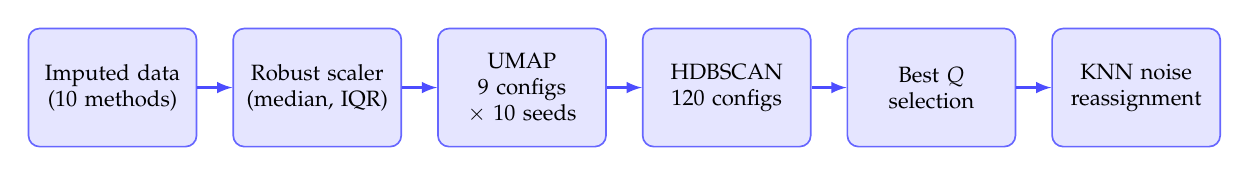
\begin{tikzpicture}[
  box/.style={draw=blue!60, line width=0.6pt, rounded corners,
              fill=blue!10, text width=1.9cm, minimum height=1.5cm,
              align=center, font=\footnotesize},
  arr/.style={->, line width=0.9pt, draw=blue!70, >=latex}
]
  \node[box] (imp) at (0,0)    {Imputed data\\(10 methods)};
  \node[box] (std) at (2.6,0)  {Robust scaler\\(median, IQR)};
  \node[box] (umap) at (5.2,0) {UMAP\\9 configs\\$\times$ 10 seeds};
  \node[box] (hdb) at (7.8,0)  {HDBSCAN\\120 configs};
  \node[box] (sel) at (10.4,0) {Best $Q$\\selection};
  \node[box] (knn) at (13.0,0) {KNN noise\\reassignment};
  \draw[arr] (imp) -- (std);
  \draw[arr] (std) -- (umap);
  \draw[arr] (umap) -- (hdb);
  \draw[arr] (hdb) -- (sel);
  \draw[arr] (sel) -- (knn);
\end{tikzpicture}%
}
\caption[Pipeline overview]{This is an end-to-end clustering pipeline. Once the data have been imputed, they first pass through a robust scaler. Next, after being scaled, the imputed data pass into a UMAP hyperparameter grid with 10 random seeds for each of nine configurations, and the resulting embeddings that yield the highest silhouette value are retained. HDBSCAN then does the clustering in a 120-configuration sweep, based upon the composite quality measure $Q = \text{silhouette} \times (1 - \text{noise fraction})$, where all boundary noise points are assigned back to their respective cluster(s) via k-nearest neighbour. This entire process is run over each of the 10 possible imputation outcomes.}
\label{fig:pipeline_diagram}
\end{figure}

\subsection{UMAP Parameter Grid}
We utilized Euclidean distance as our distance metric and \texttt{min\_dist}$=0.0$ to encourage separation between dense areas in our embedding.

\begin{table}[ht]
\caption{UMAP hyperparameter grid. All combinations of these values were put through their paces, for a total of 9 configurations.}
\label{tab:umap_grid}
\centering
\begin{tabular}{l l}
\toprule
\textbf{Parameter} & \textbf{Values} \\
\midrule
\texttt{n\_neighbors}  & 15, 30, 50 \\
\texttt{min\_dist}     & 0.0 \\
\texttt{n\_components} & 3, 5, 8 \\
\bottomrule
\end{tabular}
\end{table}

\subsection{HDBSCAN Parameter Grid}
Each UMAP embedding produced 120 possible candidate solutions (due to 120 different possible HDBSCAN configurations). To determine which configuration was "best," we employed a composite quality score that punished solutions with high silhouettes by allocating many assignments to noise:

\begin{equation}
Q = \text{silhouette} \times (1 - \text{noise proportion})
\label{eq:quality}
\end{equation}

\begin{table}[ht]
\caption{HDBSCAN hyperparameter grid. All listed value combinations were evaluated, giving me 120 configurations for each UMAP embedding.}
\label{tab:hdbscan_grid}
\centering
\begin{tabular}{l l}
\toprule
\textbf{Parameter} & \textbf{Values} \\
\midrule
\texttt{min\_cluster\_size}          & 500, 1000, 1500, 2000, 3000 \\
\texttt{min\_samples}                & 5, 10, 25, 50 \\
\texttt{cluster\_selection\_method}  & eom, leaf \\
\texttt{cluster\_selection\_epsilon} & 0.0, 0.1, 0.5 \\
\bottomrule
\end{tabular}
\end{table}

\subsection{Sweep Procedure}
The following procedures were employed for each imputed dataset: First, we preprocessed each dataset using a robust scaler. Second, we conducted a ten-fold cross-validation on each UMAP hyperparameter combination (yielding ten embeddings per combination). From these ten embeddings, we chose the best embedding based on silhouette score. Third, we conducted a 120-fold cross-validation on each HDBSCAN configuration and selected the configuration yielding the best-quality score \(Q\). Fourth, we re-labeled any observations previously labeled as noise. In doing so, noise points assigned by HDBSCAN are relocated to the nearest substantively clustered group based on k-nearest neighbor (\(k = 10\)) similarity in UMAP-space. Given that residual noise is negligible on these features, this process yields 100\% coverage and thus assigns labels to every assessment. Re-labeling is only allowed if silhouettes decrease by less than 10\%, maintaining separations between clusters.

\subsection{Worked Example}
Assume a hypothetical patient completes only those neuropsychological assessments related to orientation and digit span but fails to complete those related to Trail Making Test due to physical limitations or the delayed recall portion of the Rey Auditory Verbal Learning Test due to exhaustion. Upon application of Tier 1 filtering, however, the patient remains in the dataset with eligible variables only. The two missing scores are subsequently filled in by MICE based on observed information. The 14 variable-level scores are then subjected to winsorizing, aligned for direction, standardized, and weighted as defined in Section~\ref{sec:domain_scores} to produce six domain-composite scores. The robust scaler is applied to minimize the effect that floor and ceiling effects may have on aggregate measures. The resulting six-dimensional vector is then mapped into the cohort's UMAP representation space. The patient is then classified into one of three cognitive-severity tiers: Above Average, Near Normal, or Globally Impaired. If a patient falls into a sparse area of low density and was classified as noise, KNN reassignment utilizes neighboring assessments in UMAP-space (\(k = 10\)) and assigns them to the most closely located substantively-clustered tier. The final output includes a tier label and confidence score based on how often each imputation method agrees under hypothesis H2.

\section{Hypothesis Definitions}\label{sec:hypotheses}
\noindent \textbf{H1 (Existence of Cognitive Clusters)}. The UMAP + HDBSCAN pipeline will likely find at least two distinct, stable cognitive clusters for most imputation techniques. The existence of these clusters can be demonstrated as long as the best solution from at least 8 of the 10 different methods has both characteristics: average silhouette $\geq$ 0.40 and percentage of noisy points \(< 0.30\). Since we allow some method-specific failures, the 80\% criterion provides a margin for error.



\noindent \textbf{H2 (Robustness Across Imputation Techniques)}. Solutions for the clustering problems should show reasonable to high agreement among the imputation methods. H2 is confirmed if the median pairwise ARI and NMI for each of the $\binom{10}{2} = 45$ combinations of methods exceeds 0.50. Although there is considerable flexibility in setting this threshold, it is greater than chance and implies a substantial overlap in group membership, regardless of the degree to which individual solutions are identical.



\noindent \textbf{H3 (Relationship Between Clinical Unit \& Cluster Membership)}. Cluster membership is expected to be related to clinical unit. For each imputation technique, a contingency table is created and a chi-square test of independence is conducted. H3 is confirmed if the relationship remains statistically significant at \(\alpha = 0.05\) after a Bonferroni adjustment and Cramér's \(V > 0.10\). As a sensitivity check for potential confounds, a Cochran-Mantel-Haenszel (CMH) test is performed, conditioned on an appropriate covariate.



\noindent \textbf{H4 (Clustering at Domain-Level vs. At Variable Level)}. I expect the cognitive features at the domain level to result in a clustering representation that is more interpretable and at least as well separated as the representation based on cognitive features at the variable level. H4 will be confirmed if the domain-level approach performs at least as well as or better than the variable-level approach on at least two of three metrics: (1) higher silhouette scores; (2) lower mean VIFs; and (3) lower condition numbers. Smaller values of VIF and condition number imply less multicollinearity and better numerical conditioning. Because cross-method agreement has already been assessed in H2, comparisons of feature representations are made in H4 exclusively.

\section{Statistical Tests and Validation}\label{sec:stats}

\subsection{Statistical Conventions}
Each statistical evaluation of hypotheses follows typical statistical practice. Each evaluation assesses the data relative to a null hypothesis \(H_0\), representing a "no-effect" baseline. The p-value is the probability of obtaining a test statistic as extreme as that obtained assuming \(H_0\) to be true; smaller p-values represent stronger evidence against \(H_0\). A predetermined significance level of \(\alpha = 0.05\) serves as the threshold for rejecting \(H_0\). For any parameter, a 95\% CI represents the range that would include the population parameter in 95\% of repeated random samples from the same population using the same methodology.



For applications of bootstrapping, observed data are randomly sampled with replacement to generate a simulated approximation of the sampling distribution of a statistic. The 2.5th and 97.5th percentiles of that simulated distribution define the bootstrap CI. A z-score quantifies how many standard deviations away from the mean of a specified reference distribution a given value lies. With respect to the psychological testing instruments employed here, standardized testing permits scores derived from different instruments to be compared.



Cohen defined standards for interpreting the magnitude of effects, specifically for standardized differences, i.e., Cohen's \(d\). Specifically, \(d = 0.20\) is interpreted as a small effect size, \(d = 0.50\) as a medium-sized effect, and \(d = 0.80\) as a large effect size. When applying Cramér's V as an effect size for evaluating chi-squared tests, \(V = 0.10\) is interpreted as a small effect size, \(V = 0.30\) as a medium effect size, and \(V = 0.50\) as a large effect size.

\begin{equation}\label{eq:cohend}
d=\frac{\bar{x}_1-\bar{x}_2}{s_p},\qquad s_p=\sqrt{\frac{(n_1-1)s_1^2+(n_2-1)s_2^2}{n_1+n_2-2}},
\end{equation}

\subsection{Tests and Validation Procedures}
\noindent \textbf{Bootstrap Stability}. I conduct a bootstrap stability analysis for every imputation method using \(B = 50\) resamplings. For each resampling, I refit HDBSCAN on the cached UMAP embeddings, recording the median silhouette (Eq.~\ref{eq:silhouette}) and pre-KNN noise proportions. Pre-KNN noise proportion is equal to the proportion of observations that do not belong to any meaningful cluster:

\begin{equation}\label{eq:noise}
\text{noise}=\frac{1}{n}\bigl|\{\,i:\text{label}(i)=\text{noise}\,\}\bigr|,
\end{equation}

This is also the value used in defining quality function \(Q\) (Eq.~\ref{eq:quality}). According to H1's pre-defined conditions, a method will be deemed successful if its median silhouette is larger than or equal to 0.40 and its pre-KNN noise proportion is less than or equal to 0.30; at least 8 of the 10 methods will need to satisfy both conditions. To evaluate per-cluster stability, I apply Hennig (2007)'s matching algorithm to the pre-KNN labels using the default threshold (i.e., 0.7).



\noindent \textbf{Pairwise Agreement}. In order to remove imputation-induced variability caused by variations in other parts of pipelines, I employ a shared pipeline strategy. One StandardScaler, one UMAP model, and one k-means model are trained on MICE-imputed domain scores. The remaining methods are then standardized, projected onto this MICE-trained pipeline, and classified using that same MICE-trained pipeline. This creates the ARI (Eq.~\ref{eq:ari}) and NMI (Eq.~\ref{eq:nmi}) matrices comparing each method to each other shown as heatmaps in Chapter~\ref{Chapter4}. Confidence for each assessment is defined as:

\begin{equation}\label{eq:consensus}
\mathrm{conf}(i)=\max_{\ell}\frac{1}{M}\sum_{m=1}^{M}\mathbf{1}\!\left[\text{label}_m(i)=\ell\right],
\end{equation}

High-confidence assessments are those whose assessments were placed into the mode cluster by at least \(M/10 = 0.8 \times 10 = 8\) methods.



\noindent \textbf{Chi-Square Test, Cramér's V, CMH Test}. Contingency tables arise from cross-classifying two categorical variables - e.g., cluster assignment and clinical unit - giving joint counts. Pearson's Chi-Square Test evaluates observed counts \(O_{ij}\) against expected counts \(E_{ij}\) under the null hypothesis that the two variables are independent:

\begin{equation}\label{eq:chi2}
\chi^2=\sum_{i=1}^{r}\sum_{j=1}^{c}\frac{(O_{ij}-E_{ij})^2}{E_{ij}},\qquad E_{ij}=\frac{O_{i\cdot}\,O_{\cdot j}}{n},
\end{equation}

with \(O_{i\cdot}\) and \(O_{\cdot j}\) denoting row sums and column sums, respectively. The test statistic is referenced against a Chi-Square distribution with \((r - 1)(c - 1)\) degrees of freedom to yield the p-value. Cramér's V is used to render association statistics scale-free for sample-size purposes, since it takes on values between zero and one:

\begin{equation}\label{eq:cramersv}
V=\sqrt{\frac{\chi^2}{n\,(k-1)}},\qquad k=\min(r,c),
\end{equation}

The Cochran-Mantel-Haenszel Test extends Pearson's Chi-Square Test for data organized into strata (e.g., diagnosis subgroups). The CMH Test determines whether the association between cluster assignments and clinical units remains significant even when stratifying by an appropriate covariate:

\begin{equation}\label{eq:cmh}
\chi^2_{\mathrm{CMH}}=\frac{\bigl(\sum_{h}(a_h-\mathbb{E}[a_h])\bigr)^2}{\sum_{h}\operatorname{Var}(a_h)}.
\end{equation}



\noindent \textbf{Variance Inflation Factor}. To quantify multicollinearity in regression models, VIF is used. For any variable \(j\), it is defined as:

\begin{equation}\label{eq:vif}
\mathrm{VIF}_j=\frac{1}{1-R_j^2},
\end{equation}

where \(R_j^2\) denotes the coefficient of determination when regressing \(j\) on all other predictors. Any value exceeding 10 constitutes grounds for concern, and influences interpretation both at the variable level and in subsequent analyses at the domain level.

\subsection{Implementation}

\begin{sloppypar}
All analyses were implemented in Python (version 3.13).
Imputation used
\texttt{scikit-learn} (KNN, NMF),
\texttt{fancyimpute} (SoftImpute, EM),
\texttt{miceforest} (MICE, PMM), and
\texttt{missforest} (MissForest).
DAE and VAE used \texttt{PyTorch}.
UMAP used \texttt{umap-learn};
HDBSCAN used the \texttt{hdbscan} library.
Statistical tests used \texttt{scipy.stats} and \texttt{statsmodels}.
Validation metrics used \texttt{scikit-learn}.
The full source code, notebooks, and dashboard are available at
\url{https://github.com/zkunos/thesis_project}.
\end{sloppypar}

%----------------------------------------------------------------------------------------

% Chapter 4 (Shortened)

\chapter{Results}\label{Chapter4}

%----------------------------------------------------------------------------------------
%	SECTION 1
%----------------------------------------------------------------------------------------

\section{Exploratory Data Analysis}
Following Tier-1 filtering (Chapter~\ref{Chapter3}) and removal of all assessments lacking any cognitive measures, the remaining dataset consisted of 17{,}406 assessments from 7{,}285 patients. The resulting matrix included cognitive variables amounting to 14 variables over six domains. The percentages of missing values are provided in Table~\ref{tab:missing_descriptive}.



Data availability is inconsistent. The missingness levels vary from 0.7\% for Orientation items through to 27.8\% for ATMTA. Therefore, complete-case analysis would lose approximately half of the total clinical sample (46.9\%) and introduce clear selection bias \parencite{rubin1976inference}. Consequently, data imputation was adopted to conserve the entire clinical sample.



From a co-occurrence heatmap (not shown), blocks of variables are identified that are missing simultaneously, suggesting a missing-at-random mechanism \parencite{rubin1976inference,little2019statistical}. Dependency among missing values thus supports the application of conditional imputation rather than naive substitution. Within-domain correlation coefficients are generally high, whereas cross-domain relationships appear less prominent, suggesting common variance due to general cognitive ability \parencite{lezak2012neuropsychological}. Subsequent clustering results illustrate this common variance dimension explicitly.

\begin{table}[ht]
\caption{Missingness summary for the 14 eligible neuropsychological variables after Tier~1 filtering. The final row reports the number of complete cases (rows with no missing values across all 14 variables).}
\label{tab:missing_descriptive}
\centering
\small
\begin{tabular}{l l r r r}
\toprule
\textbf{Variable} & \textbf{Domain} & \textbf{$N$ Observed} & \textbf{$N$ Missing} & \textbf{Missing \%} \\
\midrule
\texttt{OTEMPS}          & Orientation        & 17{,}286 &   120 &  0.7 \\
\texttt{OPERSONA}        & Orientation        & 17{,}284 &   122 &  0.7 \\
\texttt{OESPAI}          & Orientation        & 17{,}282 &   124 &  0.7 \\
\texttt{ASPAN}           & Attention          & 15{,}611 & 1{,}795 & 10.3 \\
\texttt{MRAVLT075}       & Memory             & 15{,}523 & 1{,}883 & 10.8 \\
\texttt{MDIGITS}         & Memory             & 15{,}373 & 2{,}033 & 11.7 \\
\texttt{FEPMR}           & Executive Function & 14{,}682 & 2{,}724 & 15.6 \\
\texttt{LCOMPRENSIOTB}   & Language           & 14{,}686 & 2{,}720 & 15.6 \\
\texttt{LDENOMINACIOTB}  & Language           & 14{,}677 & 2{,}729 & 15.7 \\
\texttt{LREPETICIOTB}    & Language           & 14{,}634 & 2{,}772 & 15.9 \\
\texttt{MRAVLT015}       & Memory             & 14{,}281 & 3{,}125 & 18.0 \\
\texttt{MRAVLT015R}      & Memory             & 14{,}199 & 3{,}207 & 18.4 \\
\texttt{VPIMATGES}       & Visuoperception    & 12{,}992 & 4{,}414 & 25.4 \\
\texttt{ATMTA}           & Attention          & 12{,}575 & 4{,}831 & 27.8 \\
\midrule
\multicolumn{3}{l}{\textbf{Complete cases (all 14 variables observed)}} & \multicolumn{2}{r}{\textbf{9{,}245 (53.1\%)}} \\
\bottomrule
\end{tabular}
\end{table}

In Figure~\ref{fig:missingness_barplot}, missingness levels for each cognitive variable are displayed in descending order. Highly specialized assessments consistently demonstrate higher levels of missingness than routine screening measures \parencite{lezak2012neuropsychological}.

\begin{center}
\centering

\includegraphics[width=0.9\textwidth]{Figures/missingness_barplot.png}
\captionof{figure}[Missingness rates by variable]{Missingness bar plot for all cognitive variables, ordered by missingness rates. Missingness rates were higher among the specialised assessments compared to the routine screening assessments.}
\label{fig:missingness_barplot}
\end{center}

\section{Imputation Results}
Prior to conducting clustering evaluations on their respective datasets, I tested all ten imputation techniques represented in Figure~\ref{fig:imputation_comparison} and Figure~\ref{fig:imputation_comparison_b}. Due to compression of variance \parencite{rubin1987multiple}, Mean Imputation behaves differently from all other methods. All nine remaining methods maintain closer adherence to marginal distributions. Discrete structure retention is greater among donor-based methods like KNN and PMM than among model-based approaches including MICE, MissForest and EM that produce smoothed continuous reconstructions.

\begin{center}
\centering

\includegraphics[width=0.95\textwidth]{Figures/imputation_comparison_boxplots_a.png}
\captionof{figure}[Imputation comparison (ATMTA, VPIMATGES)]{Comparison of distributions for each of the 10 different imputation methods for ATMTA and VPIMATGES. Mean imputation reduces variance whereas model-based methods maintain the distributional characteristics of the original data.}
\label{fig:imputation_comparison}
\end{center}

\begin{center}
\centering

\includegraphics[width=0.95\textwidth]{Figures/imputation_comparison_boxplots_b.png}
\captionof{figure}[Imputation comparison (MRAVLT015R, MRAVLT015)]{Comparison of distributions for MRAVLT015R and MRAVLT015. Deep learning models (DAE, VAE) closely approximate model-based methods.}
\label{fig:imputation_comparison_b}
\end{center}

\section{Baseline and Primary Clustering}
I first fitted K-means and Gaussian mixture baselines across \(k=2\) through \(k=6\). Neither produced a clear discrete optimum: the K-means elbow lacked a pronounced break, and silhouette was highest at \(k=2\) but declined as additional groups were introduced. These baselines motivated examination of density structure; they were not treated as evidence that natural cognitive classes existed.

I selected HDBSCAN because it can recover irregularly shaped dense regions, represent low-density observations as noise, and examine cluster persistence across a hierarchy without requiring a fixed value of \(k\). This combination was appropriate for routine clinical data in which boundary cases may not fit cleanly into a group. UMAP was repeated across ten random seeds per parameter configuration, and HDBSCAN was evaluated over the 120-configuration grid described in Chapter~\ref{Chapter3}. The comparison of t-SNE and UMAP in Figure~\ref{fig:tsne_umap} is descriptive: it illustrates how the selected assignments appear under two projections, but it is not an independent test of cluster existence or discreteness.

\begin{sloppypar}
For the UMAP+HDBSCAN combination, the hyperparameters I settled on were: \texttt{n\_components}$=8$, \texttt{n\_neighbors}$=15$, and \texttt{min\_dist}$=0.0$ for UMAP (to allow for tight packing in the embedding space \parencite{mcinnes2018umap}); and for HDBSCAN, \texttt{min\_cluster\_size}$=1000$ and \texttt{min\_samples}$=50$ with \texttt{cluster\_selection\_method}$=\text{eom}$ and \texttt{epsilon}$=0.0$. I chose a large cluster size to ensure that only substantive groupings are retained.
\end{sloppypar}

\begin{center}
\centering

\includegraphics[width=0.9\textwidth]{Figures/tsne_umap_clusters.png}
\captionof{figure}[t-SNE and UMAP cluster projections]{Two-dimensional representations of the data using t-SNE (left) and UMAP (right), with HDBSCAN cluster assignments coloured. UMAP reveals clearer separation of cluster areas.}
\label{fig:tsne_umap}
\end{center}

\section{Cognitive Profiles of the Clusters}\label{sec:cluster_profiles}
Below are the radar plots showing mean cognitive domain score per tier, expressed as a z-score from the cohort mean. The three polygons are roughly concentric (every domain moves together), so the tiers differ in overall level rather than in profile shape.



Additionally, I created a random forest surrogate that attempts to recover the tier labels from the domain scores. The Gini importance for each domain shows which domains contribute most strongly to distinguishing among tiers. There is considerable inter-correlation between the domain scores (because they are all based on cognitive performance), so interpreting this figure requires caution: although Attention appears to have low Gini Importance relative to Working Memory and Processing Speed, for example, this may simply reflect a high degree of correlation between Attention and Working Memory rather than anything about attention being clinically unimportant.

\begin{center}
\centering

\includegraphics[width=\textwidth]{Figures/cognitive_radar_profiles.png}
\captionof{figure}[Cognitive domain severity profiles]{Left: Mean score for each cognitive domain in each tier, expressed as a z-score from the cohort mean (the dotted ring indicates the cohort average). The three polygons are approximately circular because each domain moves collectively; therefore, the tiers differ in terms of global levels rather than shapes. Right: Gini importance from a random forest surrogate that recovers tier labels from domain scores (accuracy = 0.994). Since these labels are derived from those same scores, this panel describes the decision boundaries of the partitions instead of providing independent importance measurements, and the ordering depends on inter-domain correlation (see Section~\ref{sec:feature_importance}). It should not be interpreted as suggesting that attention has no clinical significance.}
\label{fig:radar_profiles}
\end{center}

\section{Hypothesis 1: Stability and Discreteness}\label{sec:h1_results}
Hypothesis 1 contained two related claims: that reproducible groupings would be recovered and that those groupings would represent discrete cognitive phenotypes. I evaluated stability using 50 bootstrap resamples for each imputation method. HDBSCAN was refitted to each resampled UMAP embedding, and I recorded silhouette, pre-KNN noise proportion, and Hennig core-Jaccard matching. Figure~\ref{fig:h1_bootstrap} shows the bootstrap distributions, while Table~\ref{tab:h1_per_method} reports the exact per-method summaries.

\begin{center}
\centering

\includegraphics[width=0.92\textwidth]{Figures/h1_bootstrap_distributions.png}
\captionof{figure}[H1 bootstrap stability by imputation method]{Bootstrap distributions of silhouette (top) and pre-KNN HDBSCAN noise proportion (bottom) across 50 assessment-level resamples for each imputation method. Dashed lines mark the pre-specified H1 thresholds. All ten methods met the silhouette and noise criteria, although these values describe stability in the selected UMAP embedding and do not account for repeated assessments within patients.}
\label{fig:h1_bootstrap}
\end{center}

\begin{center}
\small
\captionof{table}[Per-method H1 stability results]{Exact per-method H1 results. Silhouette and noise are bootstrap medians before KNN reassignment. Overall Jaccard is the mean matched-cluster value; the final column gives the range across clusters within each method.}
\label{tab:h1_per_method}
\begin{tabular}{lrrrrr}
\toprule
\textbf{Method} & \textbf{$k$} & \textbf{Silhouette} & \textbf{Noise \%} & \textbf{Jaccard} & \textbf{Cluster range} \\
\midrule
Mean       & 4 & 0.602 &  3.4 & 0.630 & 0.627--0.633 \\
KNN        & 4 & 0.572 &  7.3 & 0.600 & 0.543--0.632 \\
MICE       & 3 & 0.581 &  7.8 & 0.573 & 0.467--0.630 \\
MissForest & 3 & 0.595 &  3.9 & 0.570 & 0.536--0.631 \\
PMM        & 4 & 0.501 &  4.0 & 0.615 & 0.580--0.631 \\
EM         & 4 & 0.571 &  7.1 & 0.509 & 0.383--0.630 \\
SoftImpute & 4 & 0.570 & 16.6 & 0.610 & 0.586--0.631 \\
NMF        & 3 & 0.543 &  3.6 & 0.584 & 0.557--0.631 \\
DAE        & 5 & 0.509 &  3.8 & 0.566 & 0.490--0.630 \\
VAE        & 4 & 0.601 & 16.0 & 0.600 & 0.574--0.631 \\
\bottomrule
\end{tabular}
\end{center}

All ten methods passed the pre-specified silhouette and noise thresholds. However, strict per-cluster reproducibility was weaker: overall core Jaccard ranged from 0.509 to 0.630, and individual matched-cluster values ranged from 0.383 to 0.633, below the conventional 0.70 stability threshold in several cases. Recovered cluster count also varied from three to five. For the MICE labels, full-coverage silhouette was 0.526 in the selected UMAP embedding but only 0.079 in the robust-scaled six-domain space. Together with the concentric profiles and dominant first principal component, these results support reproducible severity ordering but not sharply discrete natural classes. I therefore regard H1 as partially supported: stable severity bands exist, whereas discreteness does not. Because the bootstrap sampled assessments rather than patients, repeated observations may inflate apparent stability and narrow uncertainty estimates.

\section{Hypothesis 2: Imputation Sensitivity Under a Fixed Partition}\label{sec:h2_results}
Hypothesis 2 posits that different imputation methods will produce largely overlapping assignments when applied to the same incomplete data and evaluated within a fixed embedding and partition model.
The primary tiers were discovered with UMAP+HDBSCAN. For this secondary sensitivity analysis, a StandardScaler, UMAP model, and \(k\)-means labelling rule with \(k=3\) were fitted once to the MICE-imputed domain scores. Every other imputed dataset was transformed and labelled through that frozen pipeline, isolating variation in the imputed values. Across the 45 method pairs, mean ARI was 0.710 and median ARI was 0.739 (range 0.509--0.880). Mean consensus confidence was 0.929, and 86.2\% of assessments met the high-confidence definition of at least eight of ten methods agreeing.

H2 is therefore supported within its defined scope: point assignments are robust to imputation under a fixed embedding and partition. It does not follow that independently refitted UMAP+HDBSCAN pipelines recover identical density hierarchies. Full-pipeline solutions vary from \(k=3\) to \(k=5\), while five independently imputed full-pipeline runs vary from \(k=3\) to \(k=7\). This variability is compatible with discretising a continuum, but does not by itself prove that interpretation.

\begin{center}
\centering

\includegraphics[width=0.88\textwidth]{Figures/h2_ari_nmi_heatmap.png}
\captionof{figure}[ARI and NMI heatmap across imputation methods]{Adjusted Rand Index (ARI) at top and normalised mutual information (NMI) at bottom for pairwise comparisons across the 10 different imputation methods. High agreement was found throughout, although KNN showed lower agreement with the smoother model-based methods.}
\label{fig:h2_ari_nmi}
\end{center}

\begin{center}
\centering

\includegraphics[width=0.85\textwidth]{Figures/h2_consensus_confidence.png}
\captionof{figure}[Consensus clustering confidence]{Histogram of consensus confidence values under the fixed-reference H2 diagnostic. The blue reference line marks the pre-defined high-confidence threshold of 0.80, equivalent to agreement by at least eight of the ten imputation methods. Mean confidence was 0.929, and 86.2\% of assessments met this threshold.}
\label{fig:h2_consensus}
\end{center}

\begin{center}
\centering

\includegraphics[width=0.85\textwidth]{Figures/h2_method_dendrogram.png}
\captionof{figure}[Method dendrogram based on ARI distance]{Dendrogram of imputation methods using average linkage clustering on ARI-based distance metrics. KNN separates itself from other branches, and tighter grouping occurs among the smoother model-based methods.}
\label{fig:h2_dendrogram}
\end{center}

\section{Hypothesis 3: Clinical Unit Association}\label{sec:h3_results}
Hypothesis 3 tests whether cognitive-severity tier is associated with clinical-unit assignment. The chi-square test showed a statistically significant association ($\chi^2 = 911.3$, $p \approx 4 \times 10^{-156}$), with Cramér's \(V=0.162\). This is a small effect by Cohen's descriptive criteria but exceeds the pre-specified threshold of 0.10. Across five independent MICE imputations, mean Cramér's \(V\) was similar at 0.154; this is an across-imputation sensitivity summary rather than a Rubin-pooled inferential estimate.

A stratified sensitivity analysis indicated that the association remained after accounting for the broad diagnostic grouping supplied by the clinical-unit lookup. Because that grouping is derived from the same lookup as detailed unit assignment, this result should not be interpreted as independent predictive validation.

The patient-grouped multinomial sensitivity analysis provided no clear evidence that tier improved out-of-sample classification of detailed clinical unit beyond the broad diagnostic grouping. Diagnosis-only log loss was 0.6064, compared with 0.6051 after adding tier (improvement 0.0013; 95\% patient-bootstrap CI $[-0.0006,0.0031]$). Accuracy was 0.7772 versus 0.7770, and macro-F1 was 0.476 versus 0.480. I therefore conclude that H3 is supported as an association hypothesis only; the present analyses do not establish added predictive value.

\begin{center}
\centering

\includegraphics[width=0.9\textwidth]{Figures/h3_clinical_unit_heatmap.png}
\captionof{figure}[Clinical unit by cluster heatmap]{Heatmap of cluster assignments (columns) by clinical unit (rows). Cell colors represent frequencies. Specific tiers occur more frequently in certain units.}
\label{fig:h3_heatmap}
\end{center}

\section{Hypothesis 4: Feature Engineering}\label{sec:h4_results}
The main hypothesis was that domain-aggregate features would reduce redundancy and improve interpretability while retaining separation comparable to the individual variable-level representation. I compared the two representations using silhouette score, condition number, and variance inflation factors (VIFs).



Aggregate measures produced a marginally greater average silhouette score than did the individual variable-based measure (0.481 vs. 0.473; Figure~\ref{fig:h4_comparison}). More importantly, there was significant change in terms of how each set of measures conditioned the feature space. The average VIF decreased significantly, from 2.77 to 1.88, and the condition number decreased similarly, from 61.7 to 11.8. High VIFs indicate multicollinearity, which distorts computation of distances needed to perform the UMAP and HDBSCAN algorithms. Therefore, the decrease in VIFs indicates that the aggregation process reduced redundancy while maintaining the underlying cognitive constructs measured by the tests \parencite{lezak2012neuropsychological}.



Therefore, Hypothesis 4 is supported primarily through reduced redundancy and improved numerical conditioning and interpretability. The small silhouette difference does not indicate a meaningful increase in cluster separation.

\begin{center}
\centering

\includegraphics[width=0.95\textwidth]{Figures/h4_domain_vs_variable.png}
\captionof{figure}[Domain vs variable: silhouette, VIF, conditioning]{Comparison of domain-aggregated and variable-level features: silhouette (0.481 vs. 0.473), mean VIF (1.88 vs. 2.77), and condition number (11.8 vs. 61.7). Aggregation at the domain level produces similar separations but much less correlated, well-conditioned features.}
\label{fig:h4_comparison}
\end{center}

\section{Feature Importance Analysis}\label{sec:feature_importance}
To conduct this analysis, I trained a Random Forest surrogate model on the MICE-imputed Domain scores and used the tier labels as targets. It obtained an accuracy rate of 99.4\% in five-fold cross-validation. The accuracy of this surrogate model measures how well the tier labels can be predicted from the Domain scores. However, because the tier labels were created from the same Domain scores used in the clustering algorithm (UMAP + HDBSCAN), the surrogate model is essentially creating its own versions of the clustering boundaries. Therefore, since the surrogate model performs so well (i.e., nearly perfect accuracy), the tier labels demonstrate high degrees of separability in Domain space.



I employed Gini and permutation rankings to help illustrate the relative importance of each Domain. Orientation ranked highest (\(\text{Gini}=0.49\)), followed closely by visuoperceptual (\(\text{Gini}=0.24\)) and language (\(\text{Gini}=0.17\)), with attention (\(\text{Gini}=0.03\)) and executive function (\(\text{Gini}=0.02\)) last among the six domains (Figure~\ref{fig:feature_importance}). Although this order may provide some useful information about the importance of each Domain in terms of their relationships to one another, this ordering should be interpreted cautiously. It represents only what is internal to the clustering methodology and has been influenced partially by circularity. Additionally, Gini importance is biased when predictors are highly correlated \parencite{boulesteix2012overview}. As stated earlier, the six domains are highly positively correlated (both theoretically as part of the cognitive positive manifold and empirically as indicated by the first principal component in §\ref{sec:cluster_profiles}). Once a tree splits on a highly correlated Domain like orientation, attention appears redundant. Thus, even though attention ranks lowest, it is incorrect to infer that attention is clinically irrelevant. Rather, attention's position is best understood within the context of Figure~\ref{fig:radar_profiles} where the concentric profiles and principal component loadings determine whether the tiers represent total clinical severity or a Domain-specific dissociation.

\begin{center}
\centering

\includegraphics[width=0.9\textwidth]{Figures/feature_importance.png}
\captionof{figure}[Feature importance for cluster prediction]{Random Forest surrogate trained to recover tier labels from domain scores. Left: Gini importance. Right: Permutation importance with error bars. Since labels are derived from the same scores, this panel describes the decision boundaries of the clustering partitions rather than independently evaluating their relative importance. Because the domains are strongly intercorrelated, rankings should not be taken as implying clinical insignificance of attention.}
\label{fig:feature_importance}
\end{center}

\section{Robustness Analyses}\label{sec:robustness}
There are several analyses that help clarify the robustness of the hypotheses. First, I used a "listwise deletion" baseline. Second, I conducted a subsampling stability study. Third, I estimated bootstrap confidence intervals. Fourth, I compared results across independent MICE imputations. Fifth, I validated the findings using time since injury as an alternative measure. Finally, I used multiple comparison corrections for the 45 pairwise H2 tests.



\textbf{Bootstrap Confidence Intervals.} I performed a nonparametric bootstrap analysis at the assessment level. For the major estimates, I obtained very narrow 95\% confidence intervals around the estimated effects. For example, the bootstrap 95\% confidence interval for the H2 mean ARI is 0.710 [0.704, 0.716]; for H3, it is 0.16 [0.15, 0.18] (Cramér's V); and for H4, it is 0.05 [0.04, 0.06] (silhouette gap). These intervals reflect 17{,}406 assessment records, not 7{,}285 independent patients. Because follow-up assessments from the same patient were resampled independently, within-patient dependence was ignored; the intervals may therefore be too narrow and apparent stability may be inflated. They should not be interpreted as patient-level uncertainty estimates.



\textbf{H2 \& Multiple Comparison Correction.} In order to test H2, I needed to perform 45 different pairwise ARI comparisons against a cutoff of greater than 0.5. Therefore, I applied Holm-Bonferroni corrections to ensure family-wise Type I error rates, and Benjamini-Hochberg corrections to ensure false discovery rates. Using a parametric one-sided bootstrap p-value for each pair, under both types of corrections, the null is rejected for 44 of the 45 pairs; the only exception is KNN-SoftImpute (bootstrap mean \(\mathrm{ARI}=0.509\), 95\% CI [0.497, 0.521]). Thus, with respect to imputation robustness, all method pairs are significant except this one borderline case.



\textbf{Across-Imputation Sensitivity Summary.} I generated \(M = 5\) independent MICE imputations and ran the entire pipeline on each. For each nonlinear statistic, I report the across-imputation mean \(\bar{Q}\) and a descriptive dispersion interval calculated as \(\bar{Q} \pm t_{0.975,4}\sqrt{(1+1/M)B}\), where \(B\) is the sample variance of the five estimates. This calculation uses between-imputation variation only. Because no within-imputation variance was estimated, and because Cramér's V and silhouette are nonlinear statistics, these intervals are not interpreted as Rubin-rule confidence intervals. They are sensitivity summaries showing how results vary across plausible imputations. Mean Cramér's V was 0.154 with a descriptive interval of [0.049, 0.259], and the mean silhouette gap was 0.050 [0.043, 0.058]. The recovered number of clusters varied from 3 to 7, while domain-level features outperformed variable-level features in all five runs.



\textbf{Listwise Deletion Baseline.} If I discard the 46.9\% of the assessments with missing values and apply the pipeline only to the remaining 9{,}245 complete cases, I obtain two clusters with a silhouette of 0.257. Additionally, agreement between the MICE solution for those same patients and the solution based solely on complete cases is moderate (ARI 0.625, NMI 0.519), yet they are clearly not equivalent. Hence, imputation has a material impact upon the analysis: discarding the 46.9\% of the assessments with missing values changes both the quality and quantity of tiers recovered.



\textbf{Subsampling Stability.} When processing random 80\% subsamples of the cohort using UMAP+HDBSCAN, I find that the majority of samples recover the same general severity structure; however, exact labels and numbers of clusters vary from two to five. This is precisely what would be expected if I were converting a continuous gradient into discrete categories and is consistent with the per-cluster Jaccard results for H1.



\textbf{Missingness Threshold Sensitivity.} I also re-ran the entire process -- including variable selection; domain computation; MICE imputation; and UMAP+HDBSCAN -- at five Tier 1 thresholds from 30\% to 70\%. As shown in Figure~\ref{fig:sensitivity}, the solution remains in the two to three tier range with silhouettes ranging from 0.39 to 0.52 over thresholds of 40\% to 70\%. Only at 30\%, where the analysis becomes overly restrictive with regards to how many variables are allowed, does the solution break down. Therefore, the 50\% threshold used throughout the main analysis represents a reasonable balance between how much information is present in each record and how many variables are available.

\begin{center}
\centering

\includegraphics[width=0.8\textwidth]{Figures/sensitivity_analysis_a.png}\\[0.5em]

\includegraphics[width=0.8\textwidth]{Figures/sensitivity_analysis_b.png}
\captionof{figure}[Sensitivity to missingness threshold]{Effect of varying Tier~1 missingness threshold across five values (30 -- 70\%). Upper row: (a) Number of available variables and (b) Number of clusters identified. Lower row: (c) Silhouette score and (d) Proportion of noise. Vertical dashed lines indicate Tier~1 missingness threshold used in primary analyses.}
\label{fig:sensitivity}
\end{center}

\textbf{Outcome-Adjacent Validation.} Although functional outcomes are unavailable for use as validating measures of impairment status at discharge, I examined functional change through time-since-injury (TSI) at each assessment as an alternate validating measure. TSI varies significantly by tier (Kruskal-Wallis test $p = 4 \times 10^{-28}$), with median TSI times of 214 days for Above Average, 188 days for Near Normal, and 172 days for Global Impairment. Thus, as TSI increases, severity of impairment decreases across these three tiers. Among the 5{,}206 patients who have had at least two assessments, 50.2\% (2{,}613 patients) maintain their original tier assignment while 49.8\% (2{,}593 patients) experience some degree of tier shift. While such movement could suggest that patients possess a set of fixed phenotypic characteristics, such movement is far more indicative of variability in severity along a spectrum of impairment severity. Furthermore, among the 912 patients who experienced exactly two assessments and changed tiers during that period, improvement in functional status occurred approximately three times as frequently as worsening in functional status (706 vs. 206 transitions), consistent with expectations regarding natural clinical recovery patterns.



\textbf{Embedding Seed Stability.} To determine whether the clustering was due to UMAP's random initialization, I repeated the entire embedding and clustering process on the MICE-imputed domain scores using ten randomly selected seeds with equal hyperparameter settings. There was high concordance between labeling schemes; specifically, the mean pairwise ARI across the ten runs was 0.957 (median \(= 0.960\), min-max \(= [0.900, 1.000]\)). After k-nearest neighbor reassignment, this increased to 0.965. With respect to my finding that there exists a strong underlying severity axis supported by deterministic PCA (see §\ref{sec:cluster_profiles}), together with embedding seed stability, this further decreases concerns that the solution was simply an artifact of unstable UMAP initialization.



\textbf{Gaussian Mixture / Latent Profile Baseline.} As a model-based comparison, I fit Gaussian mixture models with full covariance matrices to the imputed domain scores for \(k\) varying from 2 through 6. This analysis is analogous to latent profile analysis in that it estimates model-based continuous-profile classes, but it is not a formal latent profile analysis with full-information maximum likelihood on the incomplete raw data. BIC decreased monotonically with \(k\) (from 243{,}249 at \(k = 2\) to 92{,}606 at \(k = 6\)). This shows only that no BIC optimum was reached within the tested range; it does not establish a continuum, and a solution with more than six components might have been preferred. Mixture-model solutions agreed only modestly with the density-based tiers (\(\mathrm{ARI} = 0.350-0.400\)), while the two-component solution had the clearest silhouette (0.45). I therefore treat this baseline as inconclusive about class number. The continuum interpretation rests primarily on the concentric domain profiles, the dominant first principal component, weak original-space silhouette, and sensitivity of tier count. A formal latent profile analysis with FIML and a wider class range remains a separate model-based extension.



\textbf{MNAR Tipping Point.} To establish bounds on potential missing-not-at-random mechanisms, I assumed every missing value was replaced by the worst observed performance on that variable -- either the minimum value or the maximum value depending on whether it was a timed ATMTA or not. Clearly, this is an intentionally extreme and conservative assumption. Under this condition, even though the partition became fractured and the silhouette fell to 0.030 because point-mass spikes were created when all missing values were forced to extreme values, a distinct lowest severity tier still existed and retained approximately 65.2\% of assessments originally labeled as Global Impairment. Therefore, even under extreme MNAR assumptions, Global Impairment is likely the most robust portion of the solution. Most importantly, extreme MNAR assumptions seem to degrade finer separation within lower severity tiers, and thus a formal delta-shifted tipping-point analysis seems like an interesting future direction.



\textbf{Summary Characteristics of Excluded Records.} Applying the Tier-1 filter to the full raw cohort retained 17{,}406 of the 22{,}075 records used in the source extract and excluded 4{,}669 records. Discarded records averaged only 0.800 of their 14 eligible tests, whereas retained records averaged 12.5 tests per record, thereby appearing to represent nearly empty administrative encounters instead of incomplete testing of severely impaired individuals. Demographically, both excluded records and retained records are largely indistinguishable (e.g., age at injury: 45.7 vs. 46.3 years; Cohen's \(d = -0.04\); sex: male/female = [63\%;37\%] vs. [68\%;32\%]; TSI: 2.3 vs. 1.6 years; \(d = 0.16\)). Therefore, I do not believe that the Tier-1 filter suppresses detection of a cognitively impaired subgroup identifiable via measurable characteristics -- although I cannot assess cognitive impairment directly in the excluded records.

\section{Cluster Clinical Naming}\label{sec:cluster_names}
To give the density-based clusters clinically relevant labels, I employed a rule-based naming system based upon the domain-level z-score profiles associated with each cluster.



Clustering profiles associated with domains having z-scores greater than +0.5 were labeled Above Average.



Profiles associated with domains having z-scores less than -0.5 were labeled Global Impairment.



All other profiles were labeled Near Normal.



This resulted in the final labels being Above Average ($n = 6{,}725$), Near Normal ($n = 6{,}328$), and Global Impairment ($n = 4{,}353$).



Since the tiers differ primarily in terms of overall level and not profile shape -- severity labels are preferable to phenotype names.



They provide valuable shorthand for clinicians engaged in discussing potential rehabilitation options with their patients -- as well as providing useful tier-based guidance for rehabilitation triaging efforts.



The full mapping of identifier codes to assessment frequency is contained within the interactive CogDash dashboard

% Chapter 5

\chapter{Discussion}\label{Chapter5}

%----------------------------------------------------------------------------------------
%	SECTION 1
%----------------------------------------------------------------------------------------

\section{A Cognitive Severity Gradient, Not Discrete Phenotypes}
Overall, I found no evidence of discrete cognitive phenotypes in this cohort of people with acquired brain injury (ABI); instead, I found a clear cognitive-severity gradient. I identified patients as being in the `above average', `near normal' and `global impairment' tiers based upon their performance across the battery. Importantly, these tiers differ by level, not by profile shape. As illustrated in Figure~\ref{fig:radar_profiles}, each of the six domains moves in the same direction. One principal component explained 56\% of variance in the domain scores and loaded positively across all six domains with similar magnitude. I therefore interpret the result as severity stratification rather than identification of dissociable cognitive profiles. The tiers were associated with clinical-unit placement (§\ref{sec:h3_results}), but the analysis did not establish added predictive value beyond the broad diagnostic grouping.



Moreover, my results inform a broader question in neuropsychology: whether variability across test batteries is primarily domain-specific or dominated by a general factor. I found that in this routinely collected cohort, the general severity axis accounted for most of the recoverable structure. Secondary domain-specific variation was present; however, I did not find that it determined the clustering. I interpret this pattern as consistent with both clinical experience, where global impairment often separates patients before they are differentiated further through narrow dissociations [e.g., \parencite{maas2017traumatic}], and the positive manifold of inter-test correlations found in neuropsychology \parencite{lezak2012neuropsychological}. Therefore, the phenotyping result I report here is more conservative than suggested by some other accounts. Specifically, when I analyzed the data under imputation-robust, sensitivity-tested conditions, overall severity emerged before specific patterns of profiles. I do not over-read this null result: domain aggregation and density clustering on a manifold dominated by a general factor have limited sensitivity to recover narrow dissociations, including an attention-specific subgroup, if such dissociations are small or orthogonal to the principal severity gradient.



My findings do not refute studies that report multiple dissociable cognitive profiles after brain injury (e.g., \parencite{garcia2020data}). Rather, they qualify their interpretations. Unlike those studies, my pipeline differed in several ways. For example, UMAP+HDBSCAN allows for processing of non-convex structures and low-density noise; the bootstrap analysis provided an evaluation of the replicability of the clusters; and each variable was standardized and winsorized in addition to being direction-aligned before forming aggregates. Each of these steps made a difference. High variance raw measures (i.e., a timed Trail making score) can dominate an unstandardized composite; non-cognitive variables can establish artificial axes; nearly empty records can disrupt density estimates. Thus apparent phenotypes may represent artifacts of preprocessing rather than true neuropsychological structure. Chapter~\ref{Chapter6} will examine this relationship further.



I regard H1 as partially supported (§\ref{sec:h1_results}). All ten imputation methods met the pre-specified silhouette and noise criteria, supporting recovery of ordered severity bands. However, overall core Jaccard ranged from 0.509 to 0.630, individual matched-cluster values ranged from 0.383 to 0.633, and the number of recovered groups varied from three to five. These results do not support sharply discrete, uniformly reproducible phenotypes. Boundary movement can occur without disrupting the underlying severity order.



Therefore, I argue that the three-tier solution developed from the primary MICE pipeline should be viewed as an interpretable discretization of a continuum rather than as evidence of natural kinds. Other clustering techniques produce between 3 and 5 tiers depending on how they are configured. Across-imputation and threshold sensitivity analyses show that cluster counts may vary while severity ordering remains consistent. The clinically useful entity is thus the continuum; the tiers represent a convenient way to describe aspects of it.

\section{Imputation Sensitivity Under a Fixed Partition}
I regard Hypothesis 2 as the major methodological contribution, but I define its scope deliberately narrowly. I discovered the primary clusters with UMAP+HDBSCAN. For the H2 analysis, I then used a separate fixed-reference diagnostic, fitting \(k\)-means once on the MICE embedding and projecting the other imputation methods into that same structure. Under that diagnostic, point assignments changed very little with regard to imputation methods: on average, the 45 method pairs yielded a mean pairwise ARI \(> 0.70\), with 100\% yielding an ARI \(> 0.50\) (§\ref{sec:h2_results}). Therefore, I interpret the easily recoverable structure as a strong severity gradient, whereas a fragile multi-dimensional profile structure is less readily recovered. This distinction likely explains the robustness while still allowing for method-specific variability \parencite{rubin1987multiple}.



Although the imputation process influenced the number of identified tiers and the quality of those tiers, I found that the location of patients along the severity signal did not appear to depend on a particular imputation strategy. I interpret the broad implication as follows: most clinical interpretations of a patient's relative position on the severity gradient are unlikely to change solely because one defensible imputation method is substituted for another. I do not take this to mean that missing data can be handled casually. Rather, I argue that researchers should treat missingness systematically and report the method clearly, while clinicians should interpret tier labels as aids to judgement rather than as rules that replace medical training or professional experience.



As depicted in Figure~\ref{fig:h2_dendrogram}, I found a strong separation between two families of imputation methods: smooth, model-based methods (EM, DAE, and VAE) that tend to smooth towards a model based conditional mean; local donor-methods (KNN) that rely on a few local donors to plug in missing values. Although many studies use classification criteria related to whether or not an imputation method uses statistical/machine learning/deep learning families, I found the more salient divide to be between smooth and local.



At the assessment level, I found that instability correlates moderately with the fraction of imputed data (\(r = 0.47\); §\ref{sec:h2_results}). As such, I argue that downstream applications should treat assessments with heavy amounts of missing data differently from assessments that contain almost no missing data. This could be achieved by reporting decreased confidence or by comparing more than one imputation strategy.



I view consensus clustering as a practical means of addressing this issue. The ten imputation strategies align their votes regarding label assignments for individual assessments, and the resulting confidence score estimates agreement among strategies. Overall confidence is high (mean confidence 0.93; 86.2\% of assessments have high confidence). However, as I discussed previously, I interpret the lower-confidence assessments as clinically meaningful rather than merely inconvenient. Most notably, these assessments represent patients who are located near tier boundaries and should prompt caution/re-assessment.



In the literature, MICE is commonly used prior to clustering neuropsychological data. MissForest \parencite{stekhoven2012missforest} is often preferred when non-linear relationships are expected. After applying Holm-Bonferroni correction across the 45 pairs of comparison (see Section~\ref{sec:robustness}), I found that 44 of the 45 pairs reject the null hypothesis that ARI \(\leq 0.50\). Only the KNN-SoftImpute pair remains at or near threshold levels. I interpret the broader result, within the fixed-reference H2 design, as clear: the location of patients along the severity signal does not depend upon a single imputation strategy. The number of density-based tiers remains more sensitive when UMAP+HDBSCAN is refitted independently.



I also provided a listwise deletion baseline in Section~\ref{sec:robustness} to illustrate why imputation is necessary. Restricting analysis to only complete cases results in a different number of clusters and silhouette (0.257) compared to the MICE solution for shared patients (ARI 0.625). Thus, while removing the 46.9\% of assessments with missing data changes recovered structure, imputation was not merely cosmetic.

\section{Clinical Unit Association}
To determine whether the severity tiers were associated with clinical-unit assignment, I tested the contingency between tier and unit. The association was statistically significant, although the effect size was small by Cohen's standards. A stratified sensitivity analysis remained significant after accounting for the broad diagnostic grouping supplied by the unit lookup. Because this grouping and detailed unit assignment originate from the same lookup, I do not treat that result as independent validation.



The association is clinically plausible, but it is not evidence of prediction or causation. In the patient-grouped multinomial sensitivity analysis, adding tier to the broad diagnostic grouping changed held-out log loss from 0.6064 to 0.6051, with a patient-bootstrap improvement interval that included zero. Accuracy was unchanged to three decimal places. I therefore interpret H3 only as evidence that tier distributions differ across units. Whether severity tier improves prospective routing or outcome prediction requires independent predictors, patient-grouped validation, and clinical outcomes collected for that purpose.

\section{Feature Engineering}
There are many ways to define cognitive features. Two broad options are variable-level features and aggregate features. Variable-level features treat each individual test separately, whereas aggregate features represent averaged or summed versions of tests that are intended to measure a shared cognitive domain. I tested whether domain-aggregate features would be better conditioned than variable-level features. In this context, better conditioned means lower multicollinearity, indexed by smaller variance inflation factors (VIFs), and a smaller condition number.



The results supported H4. I found that domain-aggregate features were much better conditioned than variable-level features even though separation between clusters increased very little. The silhouette changed only slightly (0.481 vs. 0.473); however, mean VIF decreased from 2.77 to 1.88 and the condition number decreased from 61.7 to 11.8 (see §\ref{sec:h4_results}). I therefore interpret H4 primarily as evidence that aggregation reduces redundant information and produces a more interpretable, better-conditioned representation. It does not provide evidence of materially stronger clustering. This benefit supports the clinical practice of interpreting test batteries by domain rather than test by test \parencite{lezak2012neuropsychological}.



I emphasize one critical requirement for aggregation: preprocessing must occur before aggregation. Variables must be winsorized, direction-aligned, and standardized before they can be averaged into composites. Otherwise, differences in raw scale will produce artifacts. For example, if several memory tests are averaged without standardization, the resulting composite can be dominated by whichever test has the largest range rather than by the intended memory construct. If several highly correlated tests enter into an unstandardized composite, then UMAP and HDBSCAN can exaggerate distance computation using a common cognitive dimension. Aggregation provides one feature per construct, so each domain contributes more evenly.

\section{Feature Importance and What Drives Severity}
I view the findings presented in §\ref{sec:feature_importance} as descriptive rather than explanatory. The Random Forest surrogate produced 99.4\% accuracy using the same domain scores used to generate the labels. Thus, I interpret the ranking as primarily recovering partition boundaries rather than explanatory structures underlying those partitions. The Random Forest ranked orientation, visuoperceptual abilities, and language above attention and executive function; however, I do not give this ordering strong interpretation because the domains are highly correlated. Gini importance is susceptible to variability under correlated predictors \parencite{boulesteix2012overview}.



I consider the principal component structure more reliable. One component explained 56\% of total variance in overall cognitive severity and loaded positively with similar magnitude across all six domains. I interpret this finding as evidence that severity tiers represent general severity levels rather than domain-specific dissociations or attention-specific patterns within this particular domain-aggregated pipeline. Robustness checks presented in §\ref{sec:robustness}, including subsampling and sensitivity to missingness thresholds, suggest that severity ordering remains stable, but exact tier count depends on resolution criteria and inclusion threshold. Data-driven studies examining phenotyping should report preprocessing choices clearly and include sensitivity analyses.

\section{Clinical Implications}
I interpret the current results as consistent with a three-tier cognitive severity stratification system. However, I also identify several limits to this approach. The broad clinical implication is conservative: these tiers may help summarize relative cognitive severity, but they should not be used as stand-alone clinical rules. When patients move through the rehabilitation system, clinicians will continue to rely on medical training, local service knowledge, and professional experience when making placement decisions. At present, I do not think these results justify specific recommendations for direct clinical implementation beyond careful interpretation of cognitive severity and transparent handling of missing data.



Clinicians have long relied on visual inspection of patient distributions to identify unusual cases. I interpret the current results as supporting that practice alongside algorithmic clustering. Many assessments did not fall neatly into sharply separated clusters, and I view the central tier as especially consistent with a boundary region cut from a continuum. Because the majority of patients fall along a broad severity gradient rather than within highly separated natural categories, future tools should help identify difficult-to-cluster or boundary-near assessments rather than forcing every assessment into a definitive phenotype label.



Future researchers studying large datasets with missing cognitive data may benefit from additional diagnostics for clustering difficulty. One simple candidate is the proportion of points with very low silhouette values, for example less than 0.05, reported alongside overall silhouette and stability metrics. This would not replace substantive clinical interpretation, but it could help quantify how many assessments sit near ambiguous regions of the partition.

% Chapter 6

\chapter{Limitations and Future Work}\label{Chapter6}

%----------------------------------------------------------------------------------------
%	SECTION 1
%----------------------------------------------------------------------------------------

\section{Limitations}\label{sec:limits}
Firstly, the study was based in a single centre. All data were obtained from one rehabilitation unit. Therefore, the possibility of selection bias exists and extrapolation to other clinical groups cannot be made. Although all tests used have been extensively studied and have international validity, the six cognitive domains provide a common framework for the description of post-injury cognition. However, the validation of this cognitive severity structure will require multi-centre studies prior to its acceptance as a general characteristic of ABI rather than as a specific characteristic of this unit.


Secondly, most analyses treat 17{,}406 assessments as observations rather than grouping them within the 7{,}285 patients. Repeated follow-up assessments from one patient are correlated, yet the primary clustering and assessment-level bootstrap do not model that dependence. Retaining all assessments describes the clinical records available at different recovery stages, but it may inflate apparent cluster stability and produce confidence intervals that are too narrow. The patient-grouped multinomial sensitivity analysis avoids leakage for H3; equivalent patient-level resampling or mixed-effects validation is still needed for the primary clustering results.



Thirdly, the recovered structure is a limitation on interpretation. The major finding is a continuum rather than distinct categories. Most of the cohort fall along a single dimension representing overall cognitive severity with PC1 accounting for 56\% of the variance. The three tiers represent a discretization of this continuum. Therefore, the tiers should not be regarded as phenotypic entities with well defined boundaries. Tier count will be influenced by both the resolution of clustering and the proportion of missing data. Assessments located near tier boundaries should be viewed cautiously. Ultimately, a continuous severity score may be more representative than discrete tiers (Section~\ref{sec:future}).



Fourthly, the analytical approach has limited capacity to model temporal change. ABI recovery is typically rapid during the early stages and follows a slower rate thereafter \parencite{ponsford2014longitudinal,maas2017traumatic}. Therefore, a single assessment provides only a 'snapshot' of a patient's recovery status. For many patients in the dataset, the inclusion of multiple assessments allows for the examination of change within patients (below); however, the timing of follow-up assessments is still determined by clinical necessity rather than being standardized.



Of the 5{,}206 patients with longitudinal data (Section~\ref{sec:robustness}), the pattern described above is clinically plausible: 50.2\% of patients remain in the same tier, while of those whose tier changed, 706 moved towards improved function whereas 206 moved towards worsened function. This 3:1 ratio represents the expected direction of recovery. However, the degree to which this reflects true recovery versus selection factors (e.g., patients being discharged when they demonstrate improvement) cannot be completely distinguished.



Future longitudinal designs with standardized assessment intervals will be necessary to determine this question.



Furthermore, the imputation strategy introduces another constraint on interpretation. The MAR assumption cannot be tested from observed data alone \parencite{rubin1976inference,little2019statistical}. In clinical settings, a test may be incomplete due to the inability of a patient to complete it; therefore, the missing value may be informative and may represent impaired performance. If patterns of MNAR were prevalent in clinical settings, function might be overestimated. An upper bound on the impact of MNAR is provided by re-imputing every missing value to the lowest observed performance (the "tipping point" check; Section~\ref{sec:robustness}). Under that extreme assumption, the Global Impairment tier persisted and included 65\% of its original membership; however, the finer partition degraded. A formally-specified delta-shifted sensitivity analysis would further refine this bound.



Additionally, a structured co-occurrence of missingness may provide some reassurance regarding test-battery protocol-driven dropout rather than solely outcome-driven dropout. The comparison of 10 imputation methods also serves as a sensitivity analysis. High-confidence consensus labels were assigned to 86.2\% of assessments across methods, indicating that plausible imputation differences did not substantially affect the primary cognitive-severity structure for most of the cohort.



Another related caveat concerns the Tier-1 filter that removes assessments where more than half of their values are missing. Upon review (Section~\ref{sec:robustness}), removed records averaged only 0.8 out of 14 completed tests and were highly similar demographically to retained records. Therefore, the Tier-1 filter likely removed primarily empty administrative records rather than an undetected severely impaired group. Still, due to missing data issues, the cognitive severity of removed records cannot be assessed directly, and only the 30-70\% threshold sensitivity analysis bounds the potential effect of this decision.



Finally, the pipeline imputes and then clusters, whereas model-based alternatives exist, including latent profile analysis via full-information maximum likelihood (FIML). The Gaussian-mixture baseline in Section~\ref{sec:robustness} provides only an approximate model-based comparison because it is fitted after imputation rather than directly estimating profiles from incomplete data. Its BIC decreased through the largest tested solution, \(k=6\), which means that no optimum was identified within the tested range; this result does not itself distinguish a continuum from a model requiring more components. Thus, developing a formal latent profile analysis that uses FIML and evaluates a wider class range is another viable area of future development.



Feature-engineering remains relevant. Non-cognitive features are eliminated and every feature is standardized (direction aligned), and winsorized prior to summarizing them as composites and generating potentially artificial profile differences. More generally, the methodological lesson is clear: unsupervised phenotyping relies on preprocessing. Any distinctive phenotype identified in an exploratory fashion should be examined relative to choices about scaling, variable selection and cohort definition before it receives a clinical label.



Finally, HDBSCAN introduces sensitivity to hyperparameters. I conducted an extensive search (\(9 \times 120\) configurations) and selected optimal parameters [\texttt{min\_cluster\_size}$=1000$ and \texttt{epsilon}$=0.0$], maximizing the composite quality metric \(Q\). Because \(Q\) contains the silhouette score, and because the UMAP seed was also selected partly on silhouette performance, the reported absolute silhouette is optimistic by construction. It is best treated as a selected internal validation statistic rather than an unbiased estimate of cluster quality. Because the underlying structure is unidimensional, however, there is a relationship between cluster size and number of tiers. In addition to examining UMAP + HDBSCAN stochastically and potentially sensitively to random initialization and imperfect preservation of global structure, I applied ten random seeds per configuration/bootstrap sample/variable subset/subsampling rate combination, and PCA as an additional form of comparison. The main conclusion does not rely on UMAP alone; PCA also demonstrates that there is a strong cognitive-severity gradient (PC1 \(=56\%\)) represented by the first principal component. Re-running the entire pipeline with ten random seeds resulted in nearly identical labels (mean pairwise \(\mathrm{ARI}=0.957\); Section~\ref{sec:robustness}). While the exact number of tiers can vary slightly depending upon these checks, the overall order of severity is robust.



Lastly, computational cost presents a fourth practical limit. Running UMAP + HDBSCAN fifty times per method is computationally intensive; however, due to modularity allowing for parallel processing, runtime costs were manageable on a typical consumer-grade laptop.

\section{Future Directions}\label{sec:future}
Four potential areas for future work arise from the findings and limitations described above.



Firstly, modeling the continuum directly. The most obvious implication of the findings regarding cognitive-severity gradients is that continuous cognitive-severity indices - either derived from PCA or supervised learning models trained on functional-outcome measures - may provide more accurate representations and may be more useful summaries than tier-based classifications. Future research should investigate comparing continuous cognitive-severity indexes to tier classification schemes for predicting prognosis and for assigning rehabilitation intensity according to need by treating tier classification as an interpretable discretization of a continuous measure rather than as natural categories.



Secondly, longitudinal clustering represents an obvious next step. Applying the developed pipeline to assessments collected at regular time points would allow researchers to describe how individual patients' positions on the cognitive-severity gradient evolve over time as part of their recovery trajectories: i.e., whether patients' initial levels predict longer-term outcomes and whether recovery rates differ depending on severity level \parencite{ponsford2014longitudinal}. Severity-based models describing recovery trajectories would represent much more valuable inputs to clinicians determining prognosis and rehabilitation-intensity decisions than cross-sectionally-derived assessments.



Thirdly, multi-center validation represents an essential requirement for considering cognitive-severity stratification as a feature of acquired-brain injury rather than as a feature of this specific service. A multi-center study across different health care systems would assess whether the one-dimensional cognitive-severity gradient found here survives changes in catchment population, test batteries, and assessment schedules \parencite{maas2017traumatic}.



Fourthly, integrating neuroimaging will help link cognitive-severity gradings with neural mechanisms. By correlating an individual's position on the cognitive-severity gradient to structural-functional imaging metrics, researchers may identify the neural correlates of global cognitive impairments following ABI; this type of evidence may assist in targeting interventions \parencite{saatman2008classification,maas2017traumatic}.

% Chapter 7

\chapter{Conclusions}\label{Chapter7}

%----------------------------------------------------------------------------------------
%	SECTION 1
%----------------------------------------------------------------------------------------

\section{Summary of Key Findings}
The purpose of this study was to find out if data-driven clustering of neuropsychological testing could show a cognitive pattern in acquired brain injury (ABI) that would be reliable, understandable and useful to clinicians. Four hypotheses were tested using a pipeline that consisted of UMAP dimensionality reduction, HDBSCAN density-based clustering, and multiple imputation methods for missing clinical data.



Overall, the major finding of this research was that the cognitive structure found through the clustering process represents a cognitive severity gradient, not a distinct number of phenotypes. The cohort represents a single dimension of overall cognitive severity. The first principal component accounts for approximately 56\% of the total variability among the six cognitive domains, with almost identical positive weights. The pipeline takes this continuum and divides it into three tiers: Above Average (38.6\%, \(n = 6{,}725\)), Near Normal (36.4\%, \(n = 6{,}328\)), and Globally Impaired (25.0\%, \(n = 4{,}353\)). The level determines which tier a participant falls into. However, there is no evidence that shape affects this outcome.



Hypothesis 1 is supported with an important caveat. There are identifiable clusters that are relatively stable. However, these are best viewed as severity bands. Each of the ten imputation methods meets the pre-specified silhouette and noise thresholds, and the two extreme tiers remained fairly consistent under Hennig per-cluster matching (Core Jaccard 0.63 and 0.62, respectively; §\ref{sec:h1_results}).



Hypothesis 2 is also supported. Using a common pipeline, the average Adjusted Rand Index across all forty-five pairwise method comparisons is .710 (95\% bootstrap CI [.704, .716]), greater than the .500 threshold. Following Holm-Bonferroni adjustment, forty-four of forty-five pairwise combinations reject \(H_0: \mathrm{ARI} \leq .5\) at \(\alpha = .05\). Only KNN-SoftImpute is borderline. Consensus clustering achieves a mean confidence of .929, with 86.2 percent of assessments receiving high-confidence assignment. The baseline comparison with listwise deletion verifies that imputation is analytically required: removing missing values from 46.9 percent of the assessments alters the number of clusters and lowers the silhouette value to .257.



Hypothesis 3 is supported as well. Clinical Unit is significantly correlated with cognitive severity tier ($\chi^2 = 911.3$, $p \approx 4 \times 10^{-156}$); however, the magnitude of the correlation is small (Cramér's \(V = .162\)). The Cochran-Mantel-Haenszel statistic demonstrates that clinical unit is not solely determined by diagnosis group \parencite{cochran1954some}. Thus, cognitive severity appears to contribute to clinical unit designation independently of diagnostic category.



Lastly, Hypothesis 4 is supported. Domain-level aggregation generates cluster separation comparable to variable-level features (silhouette .481 vs. .473), and domain-level aggregation also decreases multivariate collinearity (mean VIF 1.88 vs. 2.77) and increases numerical stability (11.8 vs. 61.7). These results provide empirical support for conceptualizing cognitive performance at the domain level.

\section{Methodological Contribution}
There are two methodological contributions made within this dissertation. First, an imputation-robustness framework is presented. The combination of ARI/NMI comparison and consensus confidence measures provides a systematic means to evaluate whether differences in clustering result arise due to differing missing-value algorithms. Due to its domain-agnostic nature, the framework may be employed with other types of partially observed clinical or biomedical data, including genomic data or survey responses.



Second, a cautionary note is provided regarding feature engineering. As demonstrated in this dissertation, unsupervised cognitive phenotyping is very susceptible to how features are constructed. For example, inclusion of an unintended demographic variable or failure to include any cognitive test information in the assessment record can create an artifact representing what appears to be a phenotypic grouping that in reality arises from poor construction of features. The pipeline developed in this dissertation reduces this potential source of error by excluding non-cognitive variables, ensuring that at least one cognitive variable exists for each assessment record, and performing Winsorisation, direction-alignment, and standardization on each variable prior to aggregation. Clinical labeling should occur only after these processing steps have taken place and evaluation for sensitivity.

\section{Clinical Recommendations}
Based upon these findings, I recommend the following:



\begin{itemize}

    \item Use a global severity index to supplement a diagnosis. The global severity index provides a reproducible summary description of overall cognitive function at time of assessment, regardless of the type of assessment (including imputed values for uncompleted tests). Rehabilitation teams can use both the diagnosis and a global severity index to inform their determination of appropriate treatment intensity for each patient.

\end{itemize}



\begin{itemize}

    \item Label uncertain cases instead of discarding them. Consensus clustering provides high confidence labels for 86.2 percent of assessments but about 2{,}400 assessments lie close to a tier boundary and thus will vary depending on choice of algorithm. Decision-support systems should report the confidence with which labels were generated instead of artificially confining label certainty uniformly.

\end{itemize}



\begin{itemize}

    \item Choose model-based imputation for practical use. Although MICE, EM, MissForest, and autoencoder imputation produce similarly robust results (pairwise ARI values as large as .88) compared to each other, KNN tends to behave differently from the others and Mean Imputation loses variance relative to the others. Therefore, MICE seems like a reasonable choice for practical application purposes whereas MissForest may prove useful for nonparametric modeling applications where nonlinear relationships are expected.

\end{itemize}



\begin{itemize}

    \item Develop treatment objectives at the domain level. Clustering at the domain level produces separations among clusters similar to variable-level aggregation while simultaneously reducing multivariate collinearity (mean VIF 1.88 vs. 2.77) and increasing numerical conditioning (11.8 vs. 61.7). This lends further support to the long-established neuropsychological practice of evaluating batteries according to domain of cognitive functioning \parencite{lezak2012neuropsychological}.

\end{itemize}

\section{Final Remarks}
Using a dimensional reduction technique called UMAP and clustering technique called HDBSCAN on reduced data with imputation algorithms that handle missing values, this study demonstrates that unsupervised clustering can uncover a continuous cognitive severity gradient in ABI that is robust to different imputation strategies and clinical groups and interpretable at the domain level. Furthermore, this research shows that there are no separate phenotypes in this cohort but rather a single dimension of overall cognitive severity.



Therefore, this dissertation provides empirical support for developing rehabilitation planning guidelines using severity levels for patients who have suffered an acquired brain injury. Future studies will be needed to validate the usefulness of using cognitive severity levels for rehabilitation planning purposes:



\begin{itemize}

    \item Does cognitive severity levels predict future outcomes better than diagnosis and current measures?

\end{itemize}



\begin{itemize}

    \item Would using a severity system improve resource allocation in controlled environments or is it just a formalization of what was discovered in CMH analyses?

\end{itemize}



\begin{itemize}

    \item Are there additional subgroups present in independent cohorts across multiple centers that were not evident in this sample or do they emerge due to varying characteristics of the populations sampled and/or assessment times?

\end{itemize}


%----------------------------------------------------------------------------------------
%	THESIS CONTENT - APPENDICES
%----------------------------------------------------------------------------------------

\appendix % Cue to tell LaTeX that the following "chapters" are Appendices

% Include the appendices of the thesis as separate files from the Appendices folder
% Uncomment the lines as you write the Appendices

% Appendix A

\chapter{Imputation Hyperparameters}

\label{AppendixA}

This appendix lists the hyperparameters used for each of the ten imputation methods evaluated in this thesis. Settings followed published defaults where defaults exist; remaining choices were selected by cross-validation or grid search as noted. The methods themselves are described in Chapter~\ref{Chapter3}, §\ref{sec:imputation}.

\begin{table}[ht]
\caption{Hyperparameters for the ten imputation methods.}
\label{tab:imputation_hyperparams}
\centering
\footnotesize
\renewcommand{\arraystretch}{1.2}
\begin{tabular}{@{} l p{10.5cm} @{}}
\toprule
\textbf{Method} & \textbf{Hyperparameters} \\
\midrule
Mean       & Single-pass arithmetic mean per variable. \\
EM         & Multivariate normal model; convergence $10^{-6}$; max 500 iterations. \\
MICE       & Linear regression per variable; 10 iterations; single imputed dataset for clustering. \\
KNN        & $k = 5$; inverse-distance weighting; Euclidean distance. \\
MissForest & 100 trees per forest; up to 10 iterations; variables imputed in order of increasing missingness. \\
PMM        & 5 donors; 10 iterations; implemented within the MICE framework. \\
SoftImpute & Regularisation chosen by cross-validation over 20 log-spaced values from $10^{-3}$ to $10^{2}$; convergence $10^{-5}$; max 200 iterations. \\
NMF        & Rank $r = 5$ selected by grid search over $\{2, 3, 5, 7, 10\}$; multiplicative updates; max 500 iterations. \\
DAE        & Architecture $15 \to 128 \to 64 \to 32 \to 64 \to 128 \to 15$; ReLU + batch normalisation; dropout $(0.5, 0.3)$; corruption rate 20\% with pattern-aware masking; MSE loss on observed entries; Adam optimiser ($\text{lr} = 10^{-3}$); ReduceLROnPlateau + early stopping (patience 20); 5 runs averaged. \\
VAE        & Same layer dimensions as DAE; latent dim 32; loss $= $~MSE~$+$~$\beta$-weighted KL divergence; cyclical annealing with $\beta_{\max} = 0.1$ over 40-epoch cycles; $K = 20$ latent samples averaged for final imputation. \\
\bottomrule
\end{tabular}
\end{table}

% Appendix B

\chapter{List of Abbreviations}

\label{AppendixAbbrev}

The abbreviations and acronyms used throughout this thesis are listed below.

\begin{longtable}{@{}l p{\dimexpr\textwidth-3.2cm\relax}@{}}
\textbf{ABI}        & Acquired Brain Injury \\
\textbf{ANOVA}      & Analysis of Variance \\
\textbf{ARI}        & Adjusted Rand Index (chance-corrected cluster agreement, $-1$ to $+1$) \\
\textbf{BH}         & Benjamini--Hochberg (false-discovery-rate correction) \\
\textbf{BIC}        & Bayesian Information Criterion (model-selection criterion) \\
\textbf{CI}         & Confidence interval (95\% unless otherwise stated) \\
\textbf{CMH}        & Cochran-Mantel-Haenszel (stratified association test) \\
\textbf{DAE}        & Denoising Autoencoder (deep-learning imputation) \\
\textbf{DBSCAN}     & Density-Based Spatial Clustering of Applications with Noise \\
\textbf{ELBO}       & Evidence Lower Bound (VAE training objective) \\
\textbf{EM}         & Expectation--Maximisation (maximum-likelihood imputation) \\
\textbf{FDR}        & False discovery rate (controlled by Benjamini--Hochberg) \\
\textbf{FWER}       & Family-wise error rate (controlled by Holm--Bonferroni) \\
\textbf{GAIN}       & Generative Adversarial Imputation Networks \\
\textbf{GAN}        & Generative Adversarial Network \\
\textbf{GMM}        & Gaussian Mixture Model \\
\textbf{HDBSCAN}    & Hierarchical Density-Based Spatial Clustering of Applications with Noise \\
\textbf{IQR}        & Interquartile Range (spread used by the robust scaler) \\
\textbf{KL}         & Kullback--Leibler (divergence term in the VAE loss) \\
\textbf{KNN}        & K-Nearest Neighbours \\
\textbf{KW}         & Kruskal-Wallis (non-parametric extension of one-way ANOVA) \\
\textbf{MAE}        & Mean Absolute Error \\
\textbf{MAR}        & Missing At Random \\
\textbf{MCAR}       & Missing Completely At Random \\
\textbf{MICE}       & Multiple Imputation by Chained Equations \\
\textbf{MIDA}       & Multiple Imputation using Denoising Autoencoders \\
\textbf{MLE}        & Maximum Likelihood Estimation \\
\textbf{MNAR}       & Missing Not At Random \\
\textbf{MSE}        & Mean Squared Error \\
\textbf{NMF}        & Non-Negative Matrix Factorisation \\
\textbf{NMI}        & Normalised Mutual Information (information-theoretic cluster agreement, $0$ to $1$) \\
\textbf{NN}         & Near-Normal (the middle cognitive severity tier in the MICE solution) \\
\textbf{PCA}        & Principal Component Analysis \\
\textbf{PMM}        & Predictive Mean Matching (semi-parametric imputation, runs inside MICE) \\
\textbf{RAVLT}      & Rey Auditory Verbal Learning Test \\
\textbf{RMSE}       & Root Mean Squared Error \\
\textbf{TBI}        & Traumatic Brain Injury \\
\textbf{TMT}        & Trail Making Test \\
\textbf{TSI}        & Time Since Injury (days at assessment) \\
\textbf{t-SNE}      & t-distributed Stochastic Neighbour Embedding \\
\textbf{UMAP}       & Uniform Manifold Approximation and Projection \\
\textbf{VAE}        & Variational Autoencoder (deep-learning imputation with latent sampling) \\
\textbf{VIF}        & Variance Inflation Factor (multicollinearity diagnostic) \\
\end{longtable}

%\include{Appendices/AppendixC}

%----------------------------------------------------------------------------------------
%	BIBLIOGRAPHY
%----------------------------------------------------------------------------------------

\printbibliography[heading=bibintoc]

%----------------------------------------------------------------------------------------

\end{document}  
